\documentclass[letterpaper,12pt]{article}

% @@@@@@@@@@@@@@@@@@@@@@@@@@@@@@@@@@@@@@@@@@@@@@@@@@@@@@@@@@@@>
% VALORES A MODIFICAR POR USTED:
% @@@@@@@@@@@@@@@@@@@@@@@@@@@@@@@@@@@@@@@@@@@@@@@@@@@@@@@@@@@@>

% NOTE: Leer nota en el README sobre la font.

\newcommand{\titulo}{AUTOCOMPLETADO DE CONSULTAS SPARQL, UNA ALTERNATIVA OPEN SOURCE}
\newcommand{\ciudad}{Valparaíso}
% TODO: Consultar el formato de los nombres:
\newcommand{\nombrealumno}{Carlos Andrés Ponce Godoy}
\newcommand{\nombreprofesor}{Carlos Buil}
\newcommand{\nombrecorreferente}{-}
% Mes y año del examen
\newcommand{\mesexamen}{Julio}
\newcommand{\anioexamen}{2021}
% Dedicatoria y agradecimientos
\newcommand{\dedicatoria}{
Considerando lo importancia de este trabajo para los alumnos, este apartado es para que el autor entregue palabras personales para dedicar este documento. La extensión puede ser de máximo una hoja y se deben mantener este formato, tipo y tamaño de letra.
}
\newcommand{\agradecimientos}{
Considerando la importancia de este trabajo para los alumnos, este apartado se podrá incluir en el caso de que el autor desee agradecer a las personas que facilitaron alguna ayuda relevante en su trabajo para la realización de este documento. La extensión puede ser de máximo una hoja y se deben mantener este formato, tipo y tamaño de letra.
}
\newcommand{\resumen}{
El resumen y las palabras clave no deben superar la mitad de la página, donde debe precisarse brevemente: 1) lo que el autor ha hecho, 2) cómo lo hizo (sólo si es importante detallarlo), 3) los resultados principales, 4) la relevancia de los resultados. El resumen es una representación abreviada, pero comprensiva de la memoria y debe informar sobre el objetivo, la metodología y los resultados del trabajo realizado.
}
\newcommand{\resumeningles}{
Corresponde a la traducción al idioma inglés del Resumen anterior. Sujeto a la misma regla de extensión del Resumen.
}
\newcommand{\palabrasclave}{
Cinco es el máximo de palabras clave para describir los temas tratados en la memoria, ponerlas separadas por punto y comas.
}
\newcommand{\palabrasclaveingles}{
Corresponde a la traducción al idioma inglés de Palabras Clave anteriores.
}
% @@@@@@@@@@@@@@@@@@@@@@@@@@@@@@@@@@@@@@@@@@@@@@@@@@@@@@@@@@@@>

% Paquete para importar imágenes
\usepackage{graphicx}
% Directorio de las imágenes
\graphicspath{ {figures/} }

% Idioma y fuentes
\usepackage[spanish,es-tabla]{babel}
\usepackage[T1]{fontenc}
\usepackage{fontspec}

% Paquete para definir cualquier tamaño de font
\usepackage{anyfontsize}

% Settear font
\setmainfont{Carlito}

% Tamaño de la página y márgenes
\usepackage[letterpaper,top=2.5cm,bottom=3cm,left=3cm,right=3cm,marginparwidth=1.75cm]{geometry}

% Determinar interlineado:
\renewcommand{\baselinestretch}{1.0}

% Eliminar sangrías:
\setlength{\parindent}{0cm}

% Paquete para definir los formatos de los títulos
\usepackage[explicit]{titlesec}

\titleformat{name=\section}[block]{\fontsize{16}{24}\selectfont\bfseries}{}{0pt}{#1}
\titleformat{name=\section,numberless}[block]{\fontsize{16}{24}\selectfont\bfseries}{}{0pt}{#1}
\titlespacing*{name=\section}{0pt}{0pt}{0.5cm}
\titlespacing*{name=\section,numberless}{0pt}{0pt}{0.5cm}

% Separación entre parrafos
\setlength{\parskip}{0.4cm}

% Paquetes de utilidad general
\usepackage{amsmath}
\usepackage{graphicx}
\usepackage{float}
\usepackage[colorlinks=true, allcolors=blue]{hyperref}

% Formato de las tablas de contenido
% \usepackage[tocflat]{tocstyle}
% \usepackage{tocbasic}
% \usepackage{tocstyle}
% \usetocstyle{allwithdot}

% Para obtener el número de la última página
\usepackage{lastpage}

% Header y footer
\usepackage{fancyhdr}
\fancypagestyle{portada}{
    \lhead{}
    \chead{}
    \rhead{}
    \lfoot{}
    \cfoot{\fontsize{10}{12}\selectfont \thepage}
    \rfoot{}
    \renewcommand{\headrulewidth}{0pt}
}
\fancypagestyle{intermedio}{
    \lhead{}
    \chead{\fontsize{10}{12}\selectfont\MakeUppercase{\titulo}}
    \rhead{}
    \lfoot{}
    \cfoot{\fontsize{10}{12}\selectfont Página \textbf{\thepage}\ de \textbf{\pageref{LastPage}}}
    \rfoot{}
    \renewcommand{\headrulewidth}{1pt}
}

% Comandos para secciones
\newcommand{\secnumbersection}[1]{
\addtocounter{section}{1}
\section*{CAPÍTULO \thesection \texorpdfstring{\\}\ #1}
\addcontentsline{toc}{section}{CAPÍTULO \thesection : #1}
\setcounter{subsection}{0}
}
\newcommand{\secnumberlesssection}[1]{
\section*{#1}
\phantomsection
\addcontentsline{toc}{section}{#1}
\setcounter{subsection}{0}
}

% Nombres
\addto\captionsspanish{\renewcommand{\contentsname}{ÍNDICE DE CONTENIDOS}}
\addto\captionsspanish{\renewcommand{\listfigurename}{ÍNDICE DE FIGURAS}}
\addto\captionsspanish{\renewcommand{\listtablename}{ÍNDICE DE TABLAS}}
\makeatletter
\renewenvironment{thebibliography}[1]
     {\secnumberlesssection{REFERENCIAS BIBLIOGRÁFICAS}
      \@mkboth{\MakeUppercase\bibname}{\MakeUppercase\bibname}%
      \list{\@biblabel{\@arabic\c@enumiv}}%
           {\settowidth\labelwidth{\@biblabel{#1}}%
            \leftmargin\labelwidth
            \advance\leftmargin\labelsep
            \@openbib@code
            \usecounter{enumiv}%
            \let\p@enumiv\@empty
            \renewcommand\theenumiv{\@arabic\c@enumiv}}%
      \sloppy
      \clubpenalty4000
      \@clubpenalty \clubpenalty
      \widowpenalty4000%
      \sfcode`\.\@m}
     {\def\@noitemerr
       {\@latex@warning{Empty `thebibliography' environment}}%
      \endlist}
\makeatother

% Personalizar Tabla de Contenidos

\usepackage{tocloft}
\renewcommand{\cftsecfont}{\fontsize{12}{14}\selectfont\fontspec{Carlito}}
\renewcommand{\cftsubsecfont}{\fontsize{12}{14}\selectfont\fontspec{Carlito}}
\renewcommand{\cftsubsubsecfont}{\fontsize{12}{14}\selectfont\fontspec{Carlito}}

\renewcommand\cftfigfont{\fontsize{12}{14}\selectfont\fontspec{Carlito}}

% Links sin color
\usepackage{hyperref}
\hypersetup{colorlinks = false}

% @@@@@@@@@@@@@@@@@@@@@@@@@@@@@@@@@@@@@@@@@@@@@@@@@@@@@@@@@@@@>
\begin{document}
\sloppy % Para evitar que referencias se escapen de los márgenes.

\pagestyle{portada}
\pagenumbering{roman}
% NOTE: Este archivo contiene la portada, la dedicatoria, los agradecimientos y el resumen.
% __NO ES NECESARIO MODIFICAR ESTE ARCHIVO__, esas se modifican con los comandos que aparecen en main.tex
%@@@@@@@@@@@@@@@@@@@@@@@@@@@@@@@@@@@@@@@@@@@@@@@@@@@@@@@@@@@@@@
\begin{titlepage}
\begin{center}
\noindent
{\fontsize{18}{22}\selectfont UNIVERSIDAD TÉCNICA FEDERICO SANTA MARÍA \\}
{\fontsize{16}{19}\selectfont DEPARTAMENTO DE INFORMÁTICA \\}
{\fontsize{16}{19}\selectfont \MakeUppercase{\ciudad}\ - CHILE \\}
\vspace{1.5cm}
\includegraphics[width=4.41cm,height=3.34cm]{logo/logo.jpg} \\
\vspace{1.5cm}
{\fontsize{20}{24}\selectfont ``\MakeUppercase{\titulo}'' \\}
\vfill
{\fontsize{16}{19}\selectfont \MakeUppercase{\nombrealumno} \\}
\vfill
{\fontsize{16}{19}\selectfont MEMORIA PARA OPTAR AL TÍTULO DE \\}
{\fontsize{16}{19}\selectfont INGENIERO CIVIL EN INFORMÁTICA \\}
\vspace{1.5cm}
{\fontsize{14}{17}\selectfont Profesor Guía: \nombreprofesor \\}
{\fontsize{14}{17}\selectfont Profesor Correferente: \nombrecorreferente \\}
\vspace{2.5cm}
{\fontsize{14}{17}\selectfont \mesexamen\ - \anioexamen \\}
\end{center}
\end{titlepage}

%  %@@@@@@@@@@@@@@@@@@@@@@@@@@@@@@@@@@@@@@@@@@@@@@@@@@@@@@@@@@@@@@
%  \newpage
%  \setcounter{page}{2}
%  \
%  \vfill
%  \vfill
%  \begin{flushright}
%  \noindent {\fontsize{16}{19}\selectfont \textbf{DEDICATORIA} \\}
%  \end{flushright}
%  \begin{flushright}
%  \noindent \dedicatoria
%  \end{flushright}
%  \vfill
%  %@@@@@@@@@@@@@@@@@@@@@@@@@@@@@@@@@@@@@@@@@@@@@@@@@@@@@@@@@@@@@@
%  \newpage
%  \begin{center}
%  \noindent {\fontsize{16}{19}\selectfont \textbf{AGRADECIMIENTOS} \\}
%  \end{center}
%  \noindent \agradecimientos
%  \vfill
%  %@@@@@@@@@@@@@@@@@@@@@@@@@@@@@@@@@@@@@@@@@@@@@@@@@@@@@@@@@@@@@@
%  \newpage
%  \secnumberlesssection{RESUMEN}
%  \vspace{0.3cm}
%  \noindent \textbf{Resumen---}\resumen \ \\
%  \vspace{0.3cm} \\
%  \noindent \textbf{Palabras Clave---}\palabrasclave \ \\
%  % @@@@@
%  \vspace{1.2cm} \\
%  % @@@@@
%  %\noindent {\fontsize{16}{19}\selectfont \textbf{ABSTRACT}}
%  %\vspace{1.2cm} \\
%  \secnumberlesssection{ABSTRACT}
%  \vspace{0.3cm}
%  \noindent \textbf{\emph{Abstract}---}\resumeningles \ \\
%  \vspace{0.3cm} \\
%  \noindent \textbf{\emph{Keywords}---}\palabrasclaveingles \ \\
%  %@@@@@@@@@@@@@@@@@@@@@@@@@@@@@@@@@@@@@@@@@@@@@@@@@@@@@@@@@@@@@@
%  

\newpage
\secnumberlesssection{GLOSARIO}

FIXME: ORDENAR POR ORDEN ALFABÉTICO.

Aquí se deben colocar las siglas mencionadas en el trabajo y su explicación, por orden alfabético. Por ejemplo: \\

{\setlength{\parskip}{0cm} % Para evitar saltar entre cada elemento nombrado.
%Colocar aquí siglas:
DI: Departamento de Informática.

UTFSM: Universidad Técnica Federico Santa María.

XML: FIXME.

SPARQL

RDF

URI

OWL

UNICODE

IRI

HTTP

ENDPOINT

WRAPPER

API

RIF

Ontología

Axioma

W3C

HTTPS

}


%Índice de contenidos:
\newpage
\thispagestyle{portada}
\tableofcontents

%Índice de figuras:
\newpage
\thispagestyle{portada}
\phantomsection
\addcontentsline{toc}{section}{ÍNDICE DE FIGURAS}
\listoffigures
\phantomsection
\addcontentsline{toc}{section}{ÍNDICE DE TABLAS}
\listoftables

\newpage
\pagestyle{intermedio}
\pagenumbering{arabic}
\secnumberlesssection{INTRODUCCIÓN}

SPARQL es dificil de utilizar...

Debe proporcionar a un lector los antecedentes suficientes para poder contextualizar en general la situación tratada, a través de una descripción breve del área de trabajo y del tema particular abordado, siendo bueno especificar la naturaleza y alcance del problema; así como describir el tipo de propuesta de solución que se realiza, esbozar la metodología a ser empleada e introducir a la estructura del documento mismo de la memoria.

En el fondo, que el lector al leer la Introducción pueda tener una síntesis de cómo fue desarrollada la memoria, a diferencia del Resumen dónde se explicita más qué se hizo, no cómo se hizo.


\newpage
\secnumbersection{DEFINICIÓN DEL PROBLEMA}

\subsection{La Web Semántica, RDF y SPARQL}

La Web Semántica es un conjunto de extensiones para la \textit{World Wide Web}, desarrolladas por el \textit{World Wide Web Consortium (W3C)}, las cuales buscan permitir que la información disponible en la Web pueda ser procesada de forma eficiente por máquinas \cite{berners2001semantic}. Para lograr esto, la web semántica propone agregar a la información ya existente metadatos semánticos para que estos puedan ser procesados por agentes inteligentes, los cuales, obtendrán esta información sin operadores humanos. Estos metadatos pueden ser descritos utilizando múltiples estándares existentes, uno de ellos es el \textit{Resource Description Framework (RDF)} \cite{world2014rdf}.

\textit{RDF} nos permite describir relaciones a través de trios del tipo ``\textit{Sujeto - Predicado - Objeto}'', los cuales, pueden ser representados de manera grafica a través de grafos. Un ejemplo de esto se puede apreciar en la figura \ref{fig:rdf-graph1}. En el grafo, el sujeto y el objeto son representados por vertices y el predicado, la relación entre ellos, se representa con una arista.

Cada uno de los elementos del trio corresponde a un objeto en la Web, los cuales, son identificados por Identificadores de Recursos Uniforme\footnote{Del ingles \textit{Uniform Resource Identifiers (URIs)}.}. Un ejemplo de estas \textit{URIs} es \href{http://www.wikidata.org/entity/Q1}{http://www.wikidata.org/entity/Q1} la cual identifica a ``El Universo'' en el repositorio de datos Wikidata. Sin embargo, existen ocasiones en las que no buscamos definir todo el grafo de forma constante y dejar determiados vertices o aristas en blanco, de forma tal que el grafo que estamos construyendo sea un grafo incompleto. Esto nos introduce al concepto de una variable en un grafo incompleto.


\begin{figure}[ht]
    \centering
    \includesvg[width=0.95\linewidth]{rdf-graph.svg}
    \caption{Un grafo \textit{RDF} básico.} Los nodos \textit{Subject} y
    \textit{Object} están conectados a través de la relación \textit{Predicate}.
    Fuente: \textit{RDF 1.1 Concepts and Abstract Syntax. World Wide Web
    Consortium}.
    \label{fig:rdf-graph1}
\end{figure}

Un conjunto de multiples trios nos permite construir grafos más complejos, los cuales, en conjunto con vertices variables nos permiten definir patrones de grafos, los cuales, al asignar valores concretos en sus variables generan una solución al patron representado. Un ejemplo de estos patrones se puede apreciar en la figura \ref{fig:rdf-graph-pattern-drug}.

\begin{figure}[ht]
    \centering
    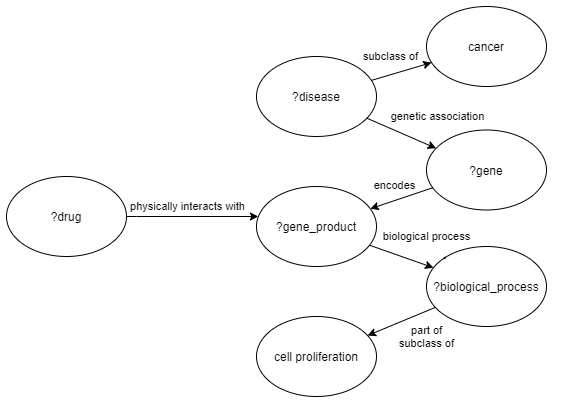
\includegraphics[width=0.95\linewidth]{graph-pattern-drug.png}
    \caption{Un grafo que representa un patron complejo.} Aquellos grafos que son solución de este patron, corresponden a aquellos medicamentos para el cáncer que afecta a los genes relacionados con la proliferación celular. Fuente: Elaboración propia.
    \label{fig:rdf-graph-pattern-drug}
\end{figure}

Estos grafos incompletos pueden ser presentados a bases de datos orientadas a grafos para ser completados a través de consultas con datos que esta base de datos en particular contiene, obteniendo así, soluciones que cumplen con el patron presentado. Existen multiples motores de bases de datos orientadas a grafos, en este trabajo nos centraremos en el repositorio de datos \textit{Wikidata} \cite{erxleben2014introducing} y su motor de busqueda \textit{Wikidata Query Service}\footnote{\href{https://query.wikidata.org/}{https://query.wikidata.org/}}.

En un ejemplo concreto, podemos obtener soluciones para el grafo de la figura \ref{fig:rdf-graph-pattern-drug} en \textit{Wikidata} a través de la consulta \textit{SPARQL} que se puede apreciar en la figura \ref{code:sparql-query-drug}. \textit{SPARQL (SPARQL Protocol And RDF Query Language)} corresponde al lenguaje estandarizado para describir consultas a repositorios de datos RDF orientados a grafos.

\subsection{Dificultades al utilizar SPARQL}

En base a todo lo anterior podemos notar lo siguiente: Para utilizar \textit{SPARQL} y obtener información util y relevante desde un repositorio \textit{RDF}, como usuarios, necesitamos dos cosas.

\begin{enumerate}
    \item Conocer la sintaxis del lenguaje para consultas \textit{SPARQL}
    \item Conocer la estructura de los elementos disponibles en el repositorio \textit{RDF}
\end{enumerate}

\begin{figure}[ht]
    \begin{lstlisting}[language=SPARQL]
    PREFIX wdt: <http://www.wikidata.org/prop/direct/>
    PREFIX wd: <http://www.wikidata.org/entity/>
        
    SELECT DISTINCT ?biological_process ?drug ?gene ?disease WHERE {
        ?gene_product wdt:P682 ?biological_process .
        ?biological_process (wdt:P361|wdt:P279)* wd:Q14818032 .
        ?drug wdt:P129 ?gene_product .
        ?gene wdt:P688 ?gene_product .
        ?disease wdt:P2293 ?gene .
        ?disease wdt:P279* wd:Q12078 .
    }
    \end{lstlisting}
    \caption{Consulta \textit{SPARQL} generada por el grafo incompleto de la figura \ref{fig:rdf-graph-pattern-drug}.} Fuente: Elaboración propia.
    \label{code:sparql-query-drug}
\end{figure}

Es bastante complicado cumplir estos prerequisitos si nuestros usuarios no tienen experiencia brevia en estas materias. Por lo tanto, para apoyar a nuestros usuarios en el proceso de cumplir sus necesidades se han desarrollado herramientas y plataformas que facilitan la construcción de consultas y la exploración de las entidades en las bases de datos \textit{RDF} como por ejemplo, \textit{RDFExplorer} \cite{vargas2019rdf}, \textit{Tabulator} \cite{berners2006tabulator} , \textit{Explorator} \cite{araujo2009experimenting}, \textit{DBpedia Atlas} \cite{valsecchi2015dbpedia}, \textit{RDF Visualizer} \cite{sayers2004node}, \textit{SPARQL Assist} \cite{mccarthy2012sparql} o \textit{YASGUI} \cite{rietveld2017yasgui}.

En este trabajo hemos decidido utilizar \textit{RDFExplorer} en base a las siguientes caracteristicas.

\begin{itemize}
    \item Facilidad de uso en su interfaz.
    \item Construcción interactiva de consultas \textit{SPARQL}.
    \item Navegación de las entidades disponibles en la base de datos \textit{RDF}.
    \item Generación de resultados parciales.
    \item Código fuente disponible y abierto \cite{vargas2019rdfrepo}.
    \item Disponible a través de una interfaz Web.
\end{itemize}

Una vista de su interfaz se puede apreciar en la figura \ref{fig:rdfexplorer}.

\begin{figure}
    \centering
    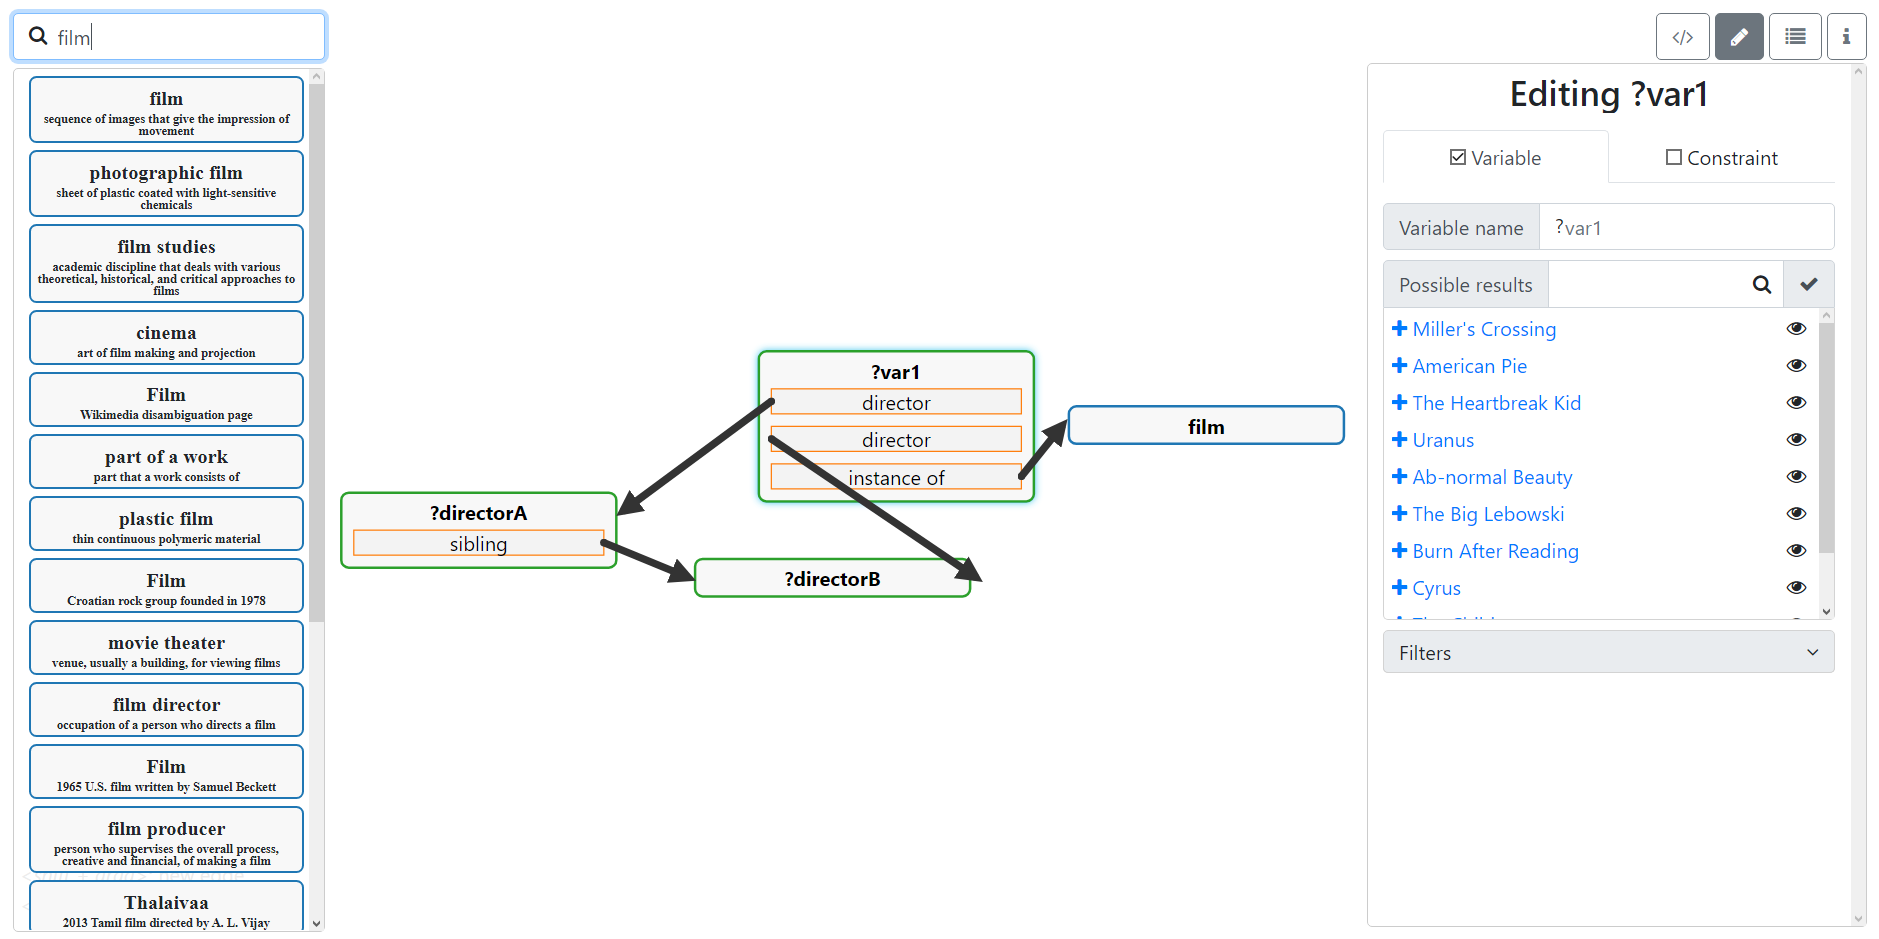
\includegraphics[width=\linewidth]{rdfexplorer.png}
    \caption{RDFExplorer, construcción de una consulta \textit{SPARQL}.} Obtiene el conjunto de aquellas películas que han sido dirigidas por hermanos. A la derecha, un conjunto de posibles resultados. Fuente: Elaboración propia.
    \label{fig:rdfexplorer}
\end{figure}

Sin embargo, aun cuando utilizamos herramientas como \textit{RDFExplorer} debemos tener algún grado de conocimiento sobre las propiedades de las entidades disponibles en nuestro repositorio \textit{RDF}. Para apoyar en esta tarea, podemos generar recomendaciones o sugerencias sobre los posibles resultados o soluciones de un grafo incompleto determiado. Esto es similar a las herramientas y funcionalidades para el autocompletado en procesadores de texto o entornos de desarrollo integrados \cite{bruch2009learning}.

\subsection{Generación de sugerencias}

En la actualidad, existen soluciones y herramientas que nos permiten obtener recomendaciones en base a consultas \textit{SPARQL} incompletas. Ejemplos de estas soluciones son \textit{Gosparqled} \cite{campinas2014live}, \textit{LinkedWiki editor} \cite{rafes2018designing}, \textit{SPARKLIS} \cite{ferre2017sparklis}, \textit{SPACE} \cite{kramer2013space} y \textit{SPARQLforHumans} \cite{parra2020autocompletion}. De las alternativas mencionadas, una tiene una importrante ventaja; \textit{SPARQLforHumans} se encuentra integrado con \textit{RDFExplorer}.

\textit{SPARQLforHumans} pareciera ser la solución a este problema, sin embargo, tiene ciertos problemas importantes descritos por sus autores.

\begin{itemize}
    \item El tiempo necesario para iniciar el software puede tomar hasta $109$ horas.
    \item Una vez iniciado el software, sus resultados son inmediatamente obsoletos. Esto, debido a que en \textit{Wikidata} pueden llegar a ocurrir $200.000$ cambios por día.
    \item El hecho de estar diseñado para soportar distintos tipos de repositorios \textit{RDF} no permite realizar optimizaciones importantes a su rendimiento.
\end{itemize}

En nuestro proyecto, vemos estos problemas como oportunidades de mejorar el rendimiento general del sistema propuesto por \textit{SPARQLforHumans}.

\subsection{Objetivos}

En base a todo lo expuesto anteriormente, en este trabajo buscamoos replicar y lograr las mismas funcionalidades generadas por el proyecto \textit{SPARQLforHumans} implementando las siguientes mejoras.

\begin{itemize}
    \item Reducir el tiempo de procesamiento para los volcados de la base de datos de \textit{Wikidata} durante el proceso de inicio del software.
    \item Implementar un mecanismo de actualización constante con los datos obtenidos directamente desde \textit{Wikidata}.
\end{itemize}

Además, vamos a definir las siguientes restricciones para nuestra solución:

\begin{itemize}
    \item Utilizaremos datos desde el repositorio \textit{RDF} \textit{Wikidata}.
    \item Utilizaremos componentes gratuitos y de código abierto para nuestro desarrollo de software.
\end{itemize}

Por ultimo, podemos definir nuestro objetivo general y objetivos especificos.

\subsubsection{Objetivo general}

Analizar, diseñar e implementar una nueva arquitectura para el proyecto \textit{SPARQLforHumans}, utilizando exclusivamente componentes de código abierto.

\subsubsection{Objetivos específicos}

\begin{itemize}
    \item Revisar y evaluar la arquitectura actual del proyecto \textit{SPARQLforHumans}.
    \item Diseñar la arquitectura del sistema utilizando solamente componentes de código abierto.
    \item Implementar la arquitectura propuesta.
    \item Evaluar el rendimiento de la solución implementada.
\end{itemize}

\newpage
\secnumbersection{MARCO CONCEPTUAL}

Para abordar nuestro problema, primero debemos definir algunos conceptos que han
sido mencionados en las secciones anteriores de forma más formal, tales como, la
\textit{web} semántica, \textit{SPARQL}, \textit{RDF} y el contexto en el que
estos se utilizan. Para esto, nos apoyaremos en las siguientes definiciones.

\subsection{\textit{Web} Semántica}

La red informática mundial, \textit{World Wide Web} o simplemente \textit{web}
es el sistema de información público más importante desarrollado en los últimos
30 años, el cual permite la transmisión de documentos electrónicos identificados
por URIs \textit{(Uniform Resource Identifiers)}, los cuales pueden estar
enlazados a otros documentos a través de hipertexto y que se encuentran
disponibles utilizando servicios de la internet.

La \textit{World Wide Web} fue diseñada como un espacio para la información con
el objetivo de no solo ser útil para las comunicaciones entre humanos, sino que
también un lugar donde las máquinas podrían ayudar y participar. Sin embargo,
uno de los principales problemas de la \textit{web} es que la mayor parte de su
contenido ha sido diseñado para ser consumido por humanos, lo que implica que
para las máquinas y el software no es fácil acceder e interpretar el contenido
disponible, incluso si este proviene de una base de datos estructurada a través
de columnas claras y tipificadas. La \textit{web} semántica busca desarrollar
herramientas, lenguajes, protocolos y estándares que permitan, tanto a maquinas
como humanos, procesar toda la información disponible en la \textit{web}. En
base a esto, podemos definir a la \textit{web} semántica como la idea de generar
una red de datos en la \textit{web}, hasta cierto punto, una base de datos
global.
\cite{berners1998semantic}

\subsection{Arquitectura de la \textit{web} semántica}

La \textit{web} semántica está construida en base a múltiples bloques, los
cuales representan estándares y lenguajes utilizados para lograr determinadas
funcionalidades descritas en su arquitectura \cite{harth2011semantic}, una
representación gráfica de esta se puede observar en la figura
\ref{fig:semantic-web-arq}, la cual, podemos describir en las siguientes capas.

\begin{figure}
    \centering
    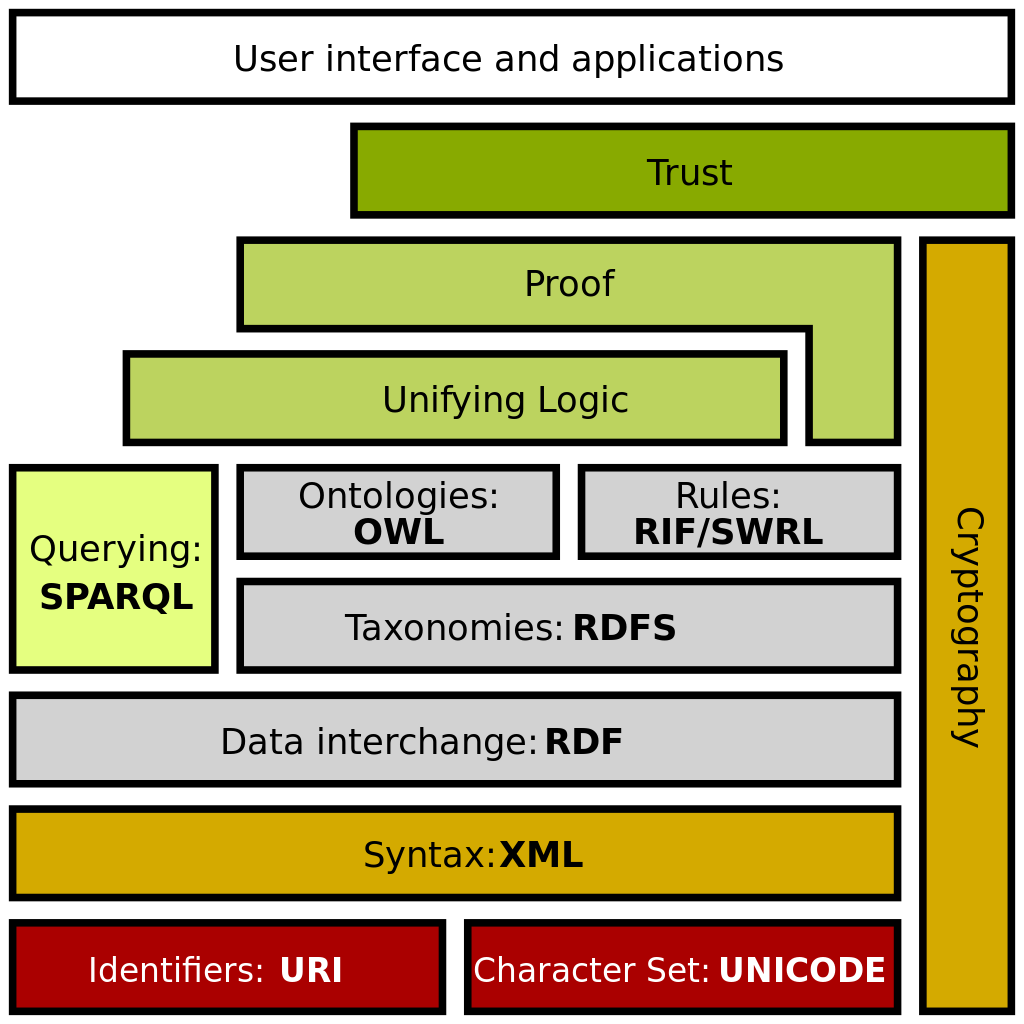
\includegraphics[width=0.6\linewidth]{semantic_web_stack}
    \caption{Arquitectura de la \textit{web} semántica.} Fuente:
    \textit{Semantic Web Stack}. Wikipedia.
    \label{fig:semantic-web-arq}
\end{figure}

\begin{enumerate}
    \item Referencias, transporte y principios de los datos enlazados.
    \item Intercambio de datos.
    \item Consultas y actualizaciones.
    \item Ontologías y razonamiento.
    \item Reglas.
    \item Seguridad y encriptación.
    \item Unificación e integración.
    \item Confianza.
    \item Aplicaciones.
\end{enumerate}

A continuación, definiremos estas capas de forma más detallada en las secciones
\ref{sec:refs-transporte-enlazados} hasta la \ref{sec:aplicaciones}.

\subsubsection{Referencias, transporte y principios de los datos enlazados}
\label{sec:refs-transporte-enlazados}

El acceso a los datos es fundamental para la arquitectura de la \textit{web}
semántica. Podemos tomar como referencia, el modelo utilizado por los servidores
\textit{web}, en el cual, los documentos disponibles se encuentran enlazados a
otros de forma descentralizada, esto es, que aquel documento referenciado no
necesariamente se encuentra en el mismo servidor que está haciendo referencia a
él. Estos enlaces, son utilizados por los usuarios para navegar entre los
millones de servidores disponibles en la \textit{web}.

Las URI/IRI y el protocolo HTTP son igual de importantes para el núcleo que
define tanto a la \textit{World Wide Web} como a la \textit{web} semántica. En
un ejemplo concreto, la URI
\url{https://en.wikipedia.org/wiki/Back_to_the_Future} en la \textit{web},
representa el documento en el servidor \url{https://www.wikipedia.org} que
contiene información sobre la serie de películas y obras de título ``Volver al
Futuro'', en cambio, en el contexto de la \textit{web} semántica, la URI
\url{https://www.wikidata.org/wiki/Q1} representa al ``universo'' como una
entidad real, la cual es parte del \url{https://www.wikidata.org/wiki/Q3327819}
``multiverso'' y es estudiado por la \url{https://www.wikidata.org/wiki/Q338}
``cosmología''.

Los datos del ejemplo anterior son publicados por ``The Wikipedia Fundation" a
través del servicio Wikidata \cite{vrandevcic2014wikidata}, pero las relaciones
descritas podrían enlazar a otros editores de contenido, como por ejemplo
DBpedia \cite{valsecchi2015dbpedia}, el cual es un esfuerzo comunitario para
extraer información estructurada desde distintas fuentes y enlazarlas a través
del formato \textit{RDF}. Para lograr esto, los editores de contenido para la
\textit{web} semántica aplican los siguientes principios a sus datos, los cuales
son conocidos como los ``principios para datos enlazados'' o
\textit{``LinkedData principles''} \cite{bizer2011linked}.

\begin{enumerate}
    \item Utilizar URIs como nombres para entidades.
    \item Utilizar URIs HTTP para que los usuarios puedan buscar y acceder a
    estas entidades.
    \item Cuando un usuario consulta una URI, debes entregar información
    relevante, utilizando estándares como \textit{RDF} y \textit{SPARQL}.
    \item Debes incluir enlaces a otras URIs, para que los usuarios descubran
    más entidades.
\end{enumerate}

\subsubsection{Intercambio de datos}
\label{sec:intercambio-datos}

\begin{figure}
    \centering
    \includesvg[width=\linewidth]{rdf-graph.svg}
    \caption{Un grafo \textit{RDF} básico.} Los nodos \textit{Subject} y
    \textit{Object} están conectados a través de la relación \textit{Predicate}.
    Fuente: \textit{RDF 1.1 Concepts and Abstract Syntax. World Wide Web
    Consortium}.
    \label{fig:rdf-graph1}
\end{figure}

Los datos de la \textit{web} semántica son generados por distintas entidades
alrededor del mundo, las cuales no están necesariamente coordinadas entre ellas,
por lo que su arquitectura debe soportar la creación distribuida de datos junto
con la integración de múltiples fuentes y la interoperabilidad entre la
información creada \cite{bizer2011linked}. Este tipo de requerimientos los
cumplen las estructuras de datos basados en grafos como \textit{RDF}.
\textit{RDF} es un formato basado en la descripción de grafos dirigidos, los
cuales representan la información de la forma de tríos ``sujeto - predicado -
objeto'', en los cuales, el sujeto y el predicado corresponden a nodos del grafo
y el predicado es un arco que los relaciona, como se puede observar en la figura
\ref{fig:rdf-graph1}. En estos tríos, cualquiera de estos objetos puede tomar el
valor de una URI, un valor literal (cadenas de texto, números o fechas) o
simplemente un nodo vacío (identificadores que no pueden ser referenciados por
otra entidad).

\textit{RDF} corresponde a la especificación de un lenguaje abstracto para
describir relaciones entre entidades, el cual, puede ser serializado en
múltiples formatos de texto como \textit{Extensible Markup Language (XML)}
\cite{beckett2004rdf} en la figura \ref{fig:rdf-xml-ex} o en un formato más
compacto llamado \textit{Turtle} \cite{beckett2014rdf} en la figura
\ref{fig:rdf-turtle-ex}.

\begin{figure}
    \centering
    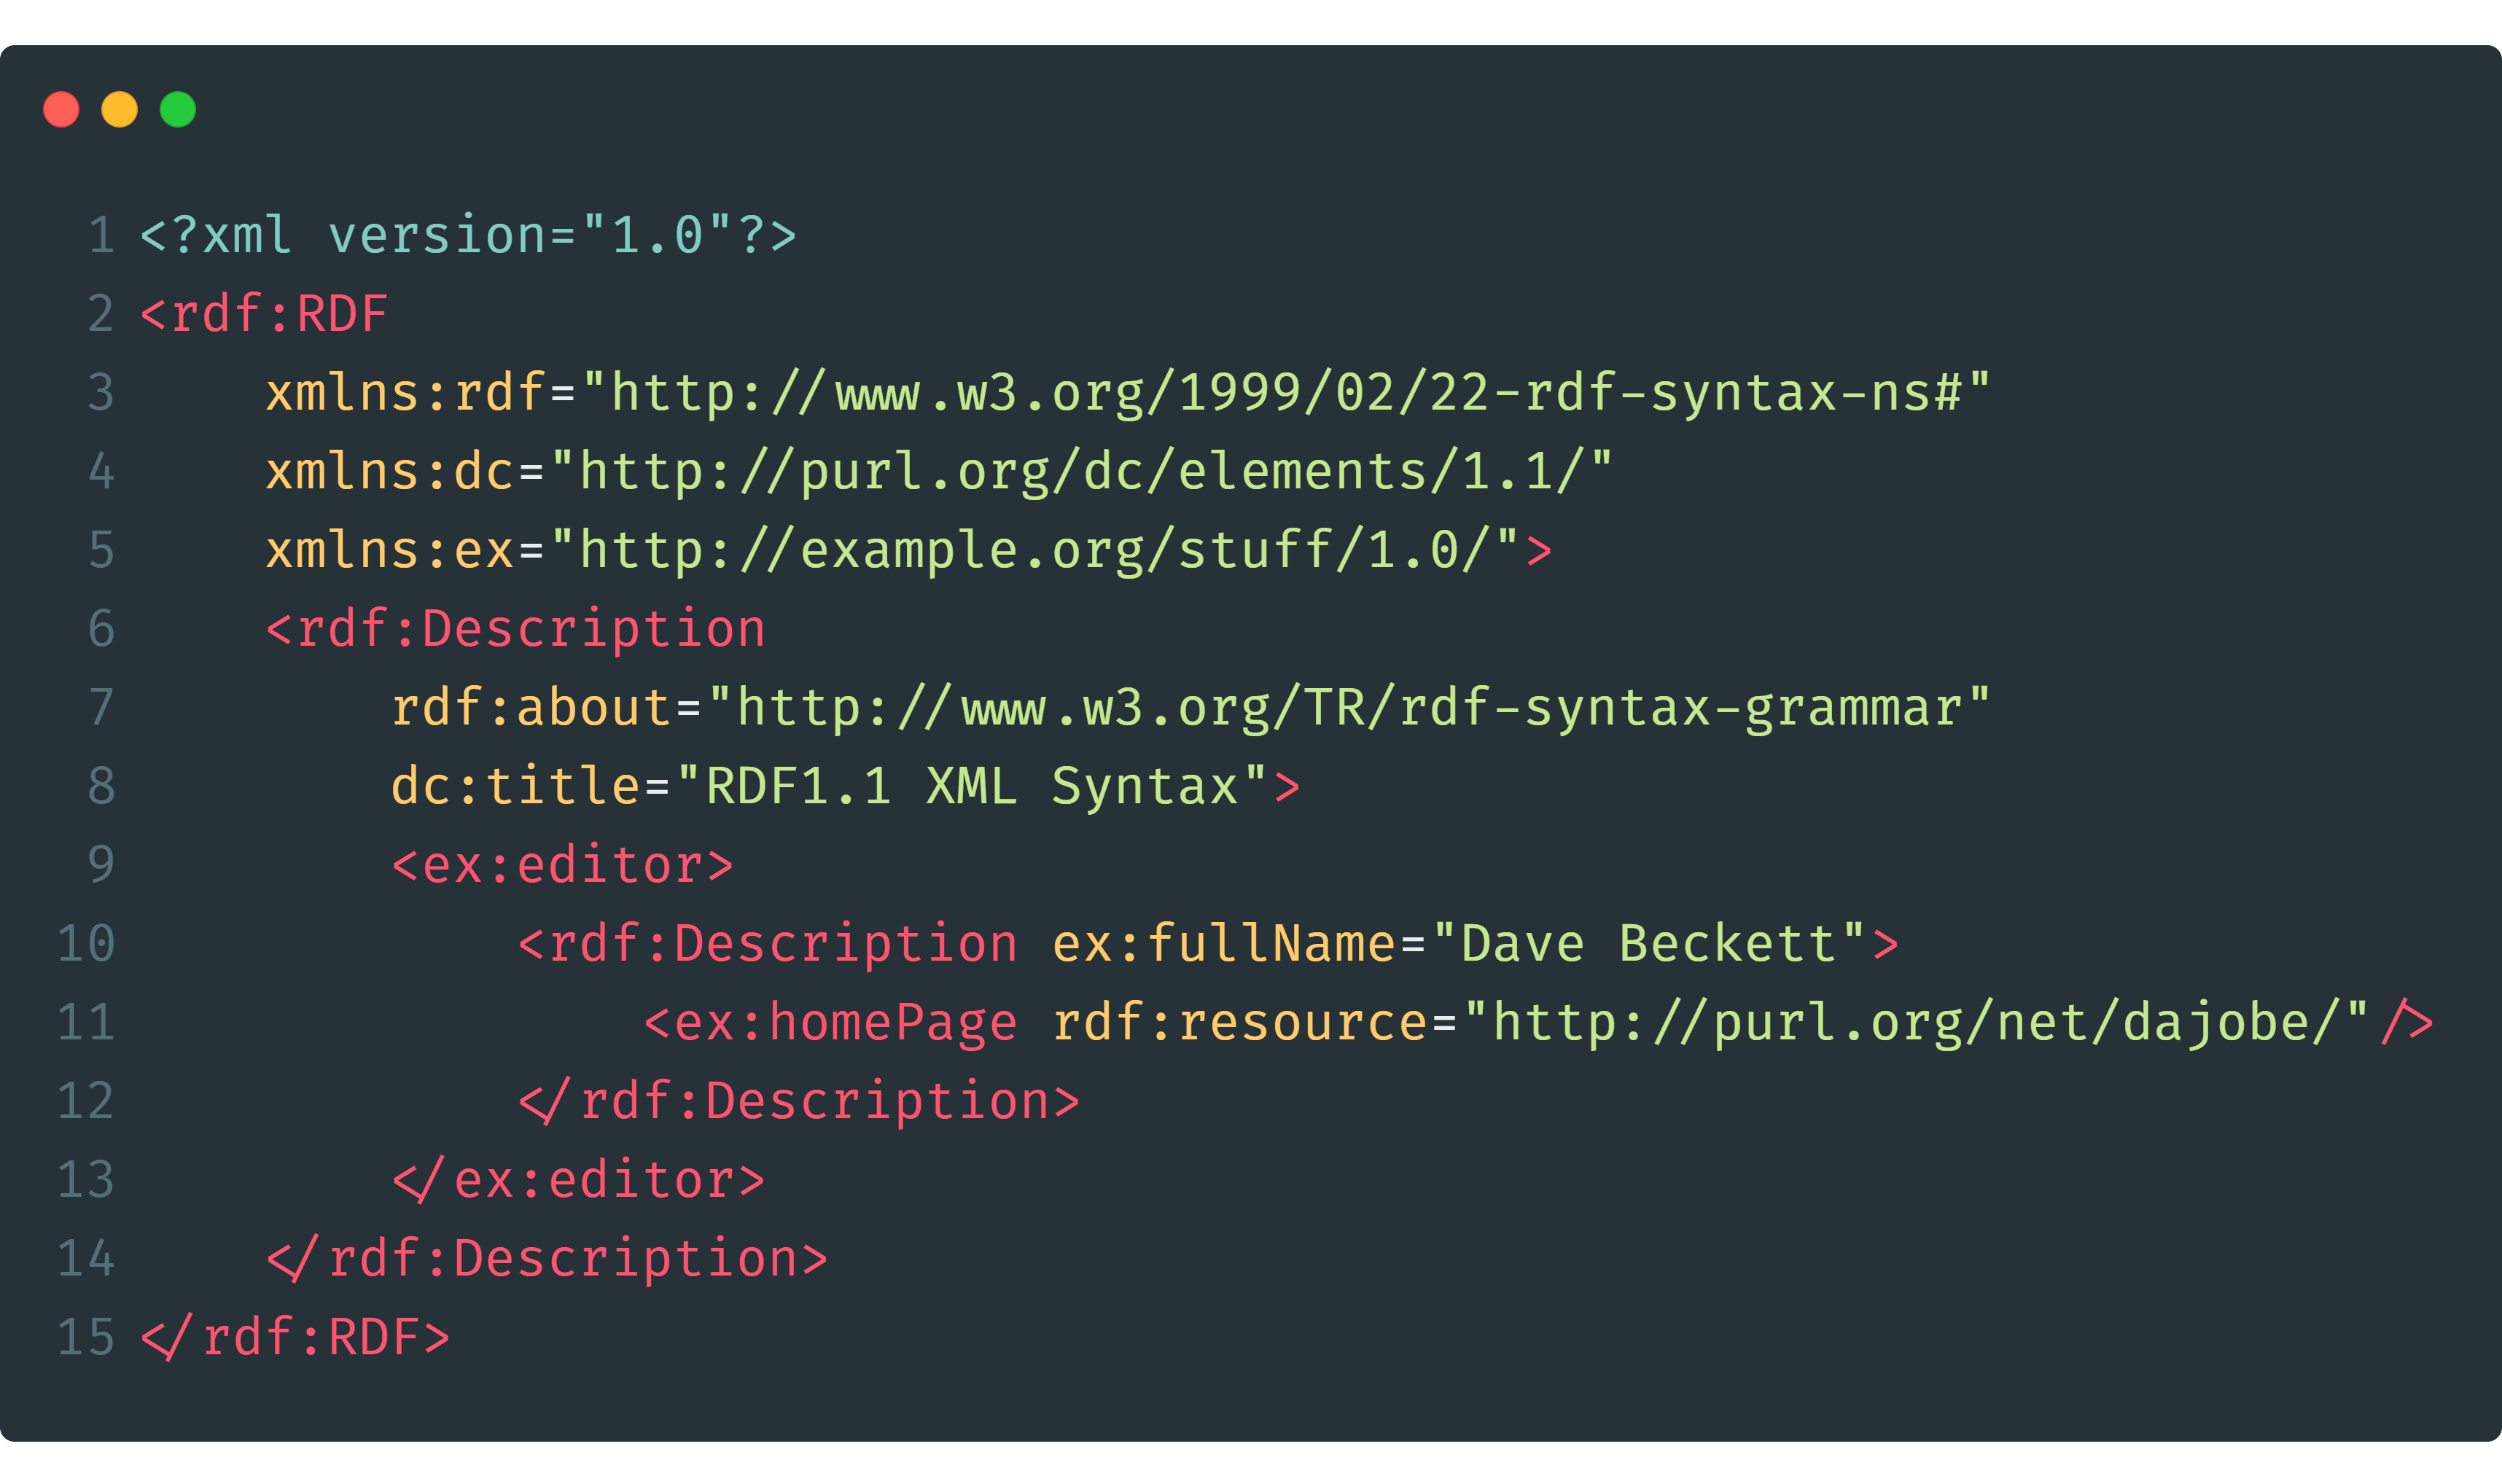
\includegraphics[width=\linewidth]{rdf-xml-ex.png}
    \caption{Descripción de un documento \textit{RDF/XML}.} Fuente: RDF 1.1 XML
    Syntax. World Wide Web Consortium.
    \label{fig:rdf-xml-ex}
\end{figure}

\begin{figure}
    \centering
    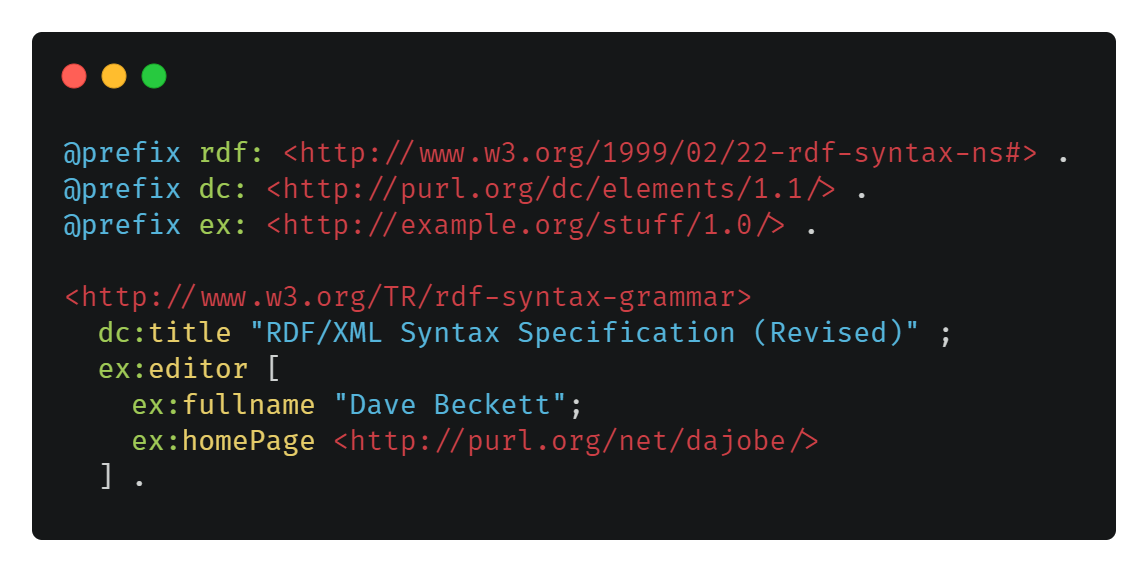
\includegraphics[width=\linewidth]{rdf-turtle-ex.png}
    \caption{Descripción de un documento \textit{RDF/Turtle}.} Fuente: Turtle
    (Syntax). Wikipedia.
    \label{fig:rdf-turtle-ex}
\end{figure}

\subsubsection{Consultas y actualizaciones}

Los principios de los datos enlazados explicados en la sección
\ref{sec:intercambio-datos} nos entregan guías sobre cómo realizar la
publicación y permitir el acceso a datos simples, sin embargo, no es posible
realizar consultas complejas a aquellos datos publicados utilizando estos
principios, puesto que, no es necesario contar con un sistema o mecanismo de
consulta para publicar información. Si continuamos con el ejemplo de las
películas ``Volver al Futuro'', consideremos que buscamos obtener los títulos de
aquellas películas en las que los miembros del elenco de ``Volver al Futuro''
también han actuado. Una forma relativamente sencilla de lograr esto, es acceder
a la URI que representa la película, obtener las URIs de los actores y de forma
iterativa acceder a estas URIs para obtener el nombre de las películas en las
que cada miembro ha participado. No es difícil darse cuenta, que este proceso no
es para nada eficiente en tiempo de ejecución ni recursos de red utilizados.

Para resolver esta consulta, utilizamos el lenguaje de consultas para
repositorios \textit{RDF} llamado \textit{SPARQL}, cuyo nombre corresponde al
acrónimo recursivo ``\textit{\textbf{S}PARQL \textbf{P}rotocol \textbf{A}nd
\textbf{R}DF \textbf{Q}uery \textbf{L}anguage}'' \cite{world2013sparql}. Este
lenguaje está diseñado para evaluar consultas en repositorios de datos que están
almacenados en formato \textit{RDF}, en estos repositorios, la información no se
obtiene accediendo de forma iterativa a distintas URIs que representan
entidades, si no que enviando consultas a un
\textit{endpoint}\footnote{\textit{Endpoint:} Del inglés punto final. Se refiere
a un punto en la red expuesto por un sistema informático con el cual se puede
interactuar o establecer un canal de comunicaciones.} que soporta
\textit{SPARQL}. \textit{SPARQL} permite a sus usuarios especificar URIs
arbitrarias, las cuales podrían no ser accesibles a través de la \textit{web},
junto con un patrón de grafo dirigido el cual debe coincidir con los datos
disponibles en el repositorio y en el que pueden ser descritas determinadas
restricciones para los datos obtenidos. En la figura \ref{fig:graph-pattern-ex}
se puede apreciar el patrón del grafo utilizado para consultar por las películas
en las que el elenco de ``Volver al futuro'' ha participado.

\begin{figure}
    \centering
    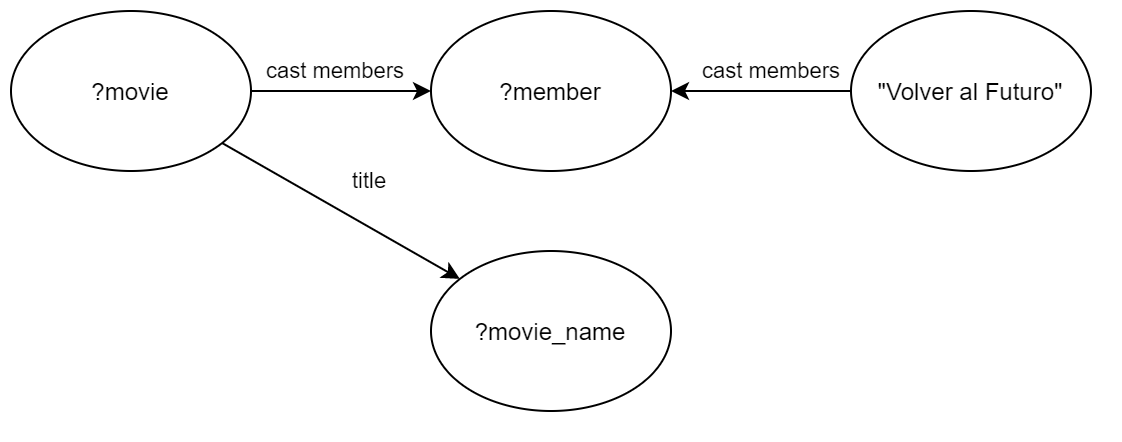
\includegraphics[width=\linewidth]{graph-pattern-ex.png}
    \caption{Patrón de un grafo \textit{RDF} básico. } Fuente: Elaboración
    propia.
    \label{fig:graph-pattern-ex}
\end{figure}

Esta consulta puede ser representada utilizando \textit{SPARQL}, como se puede
apreciar en la figura \ref{fig:graph-pattern-ex-sparql}. Una consulta
\textit{SPARQL} está compuesta de múltiples secciones, las sentencias
\textit{\texttt{PREFIX}} son utilizadas para abreviar URIs y su rol es apoyar la
legibilidad de la consulta. El núcleo de una consulta se encuentra en la sección
\textit{\texttt{WHERE}}, en la cual, se debe definir de forma precisa el patrón
de nuestro grafo dirigido, el cual debe coincidir con la información semántica
disponible. Un grafo básico consiste en patrones individuales los cuales pueden
ser sujetos, predicados u objetos unidos por variables, formando una plantilla,
la cual será completada en el proceso de evaluación de la consulta. De forma
opcional, una sentencia \textit{\texttt{WHERE}} puede estar acompañada de una
expresión \textit{\texttt{FILTER}} la cual puede acotar los resultados obtenidos
a determinadas estructuras que cumplan con criterios especificados.

\begin{figure}
    \centering
    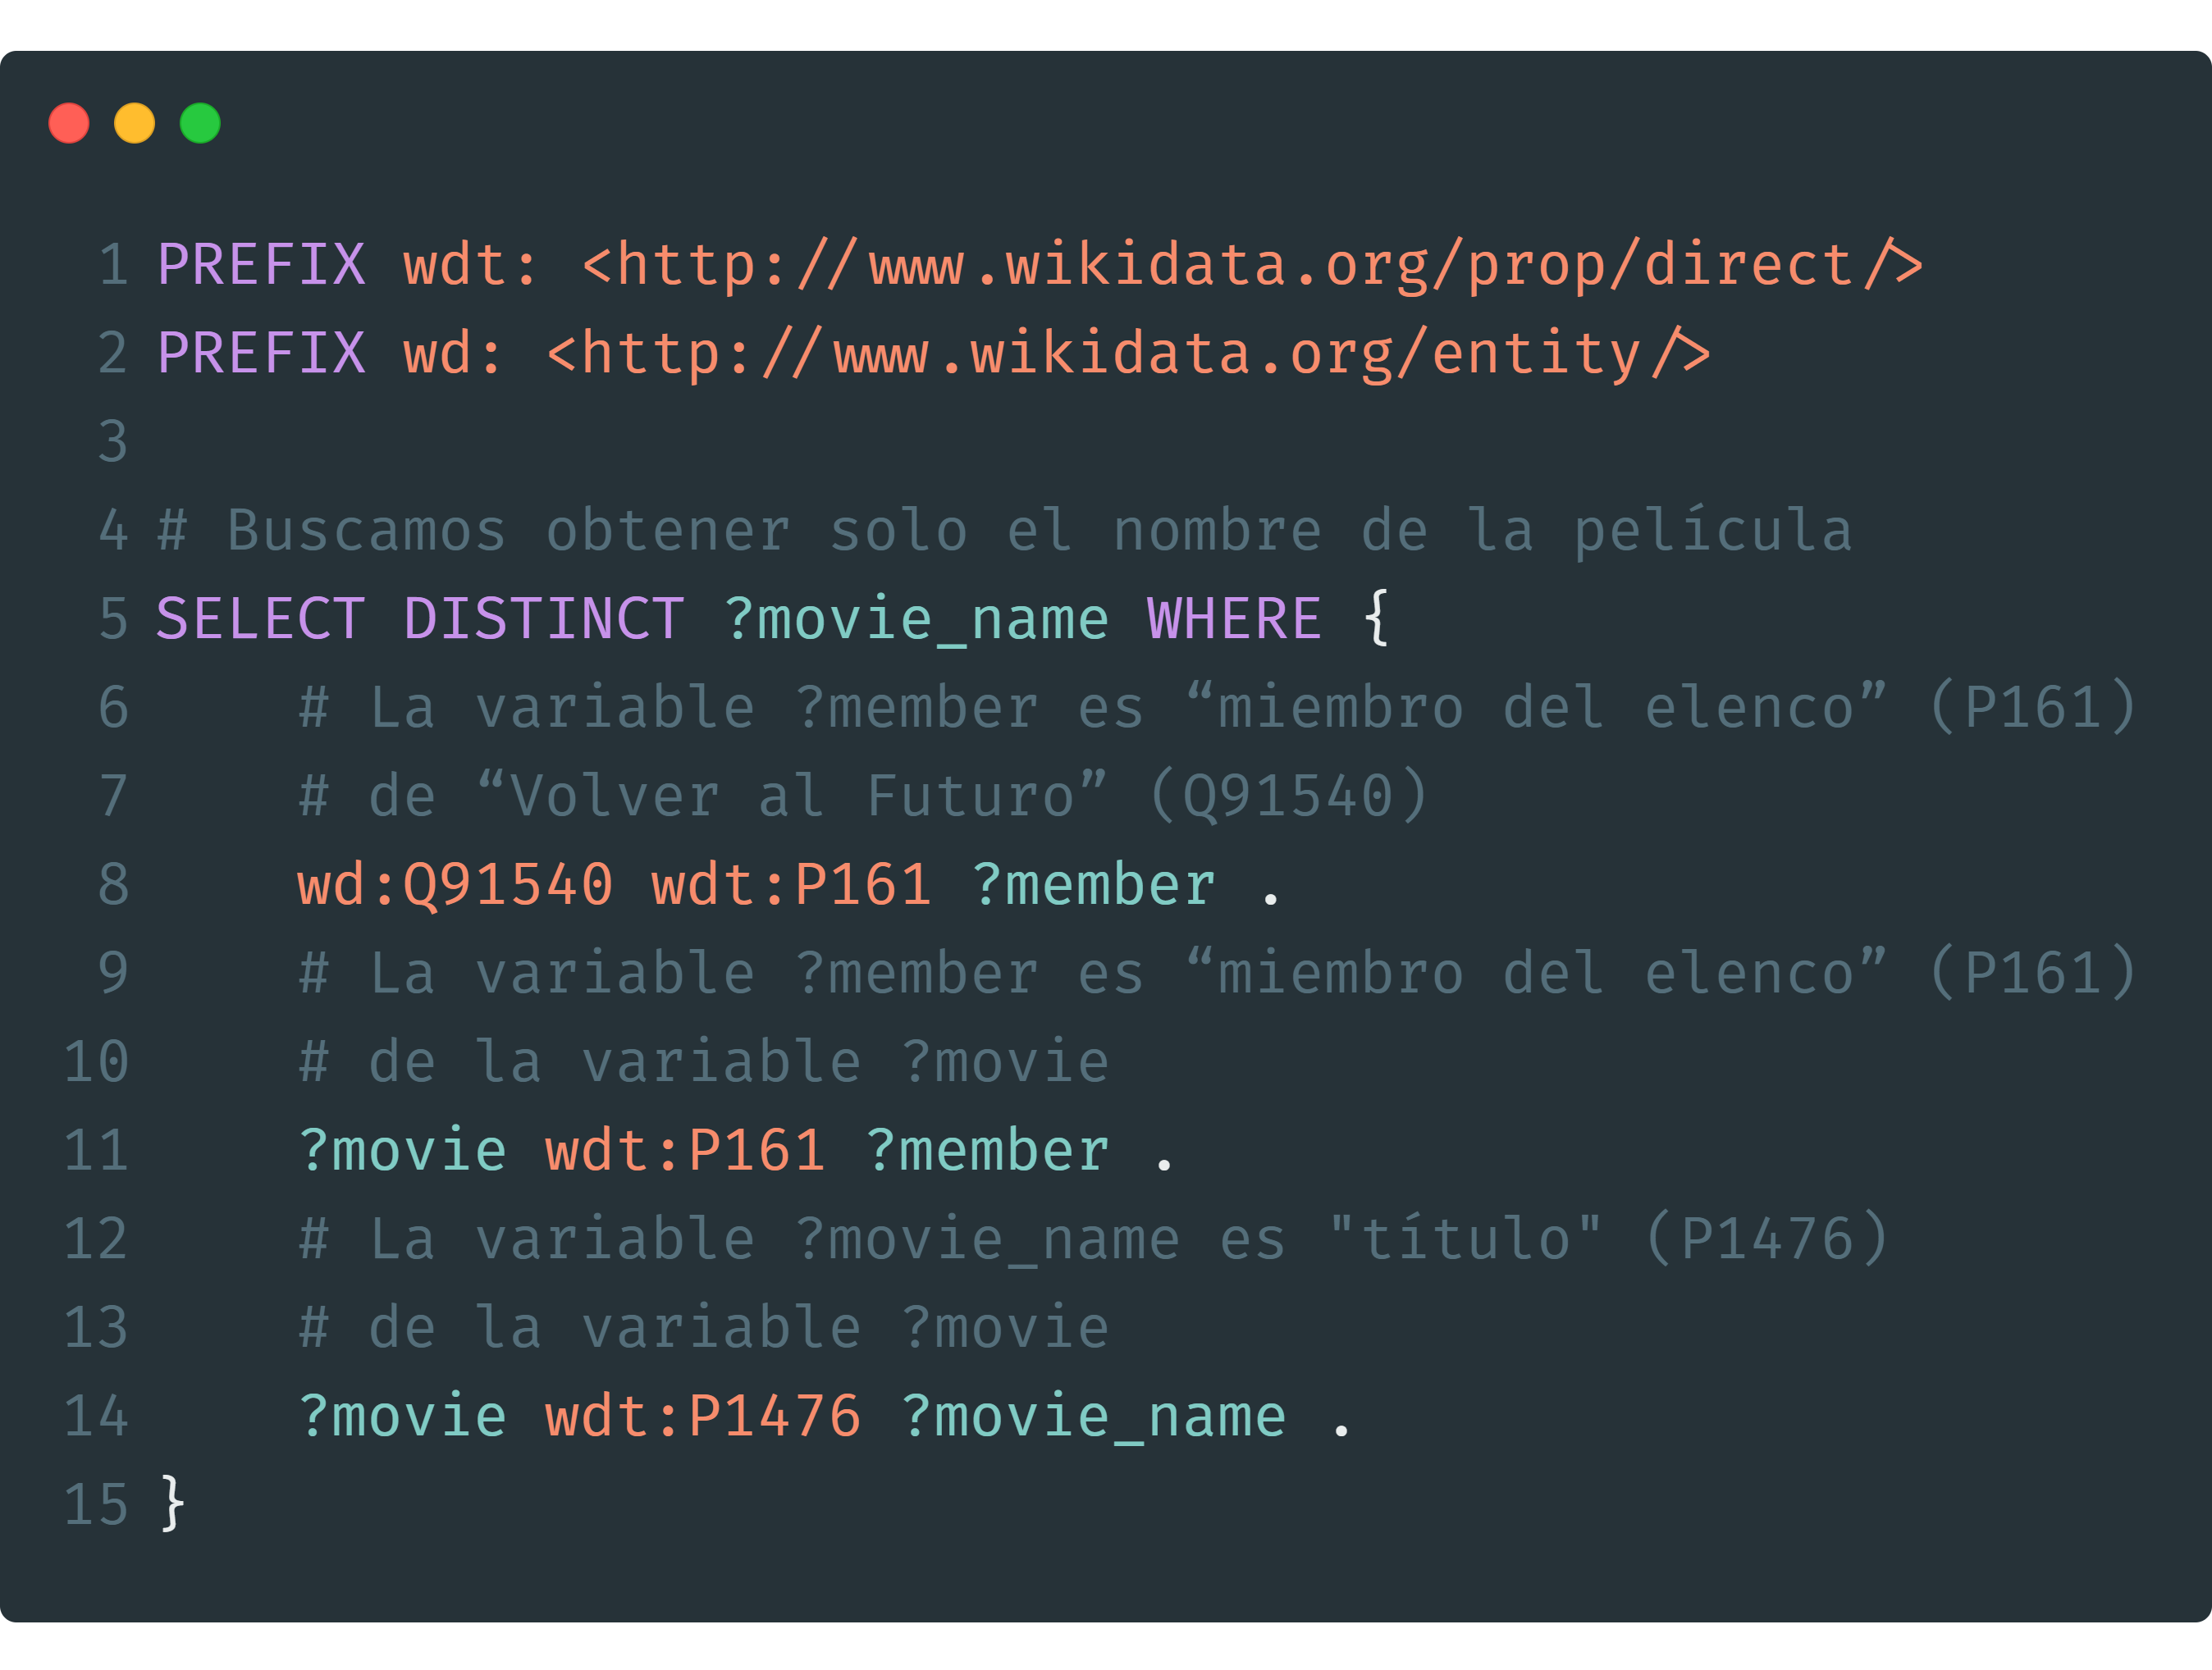
\includegraphics[width=0.85\linewidth]{graph-pattern-ex-sparql.png}
    \caption{Una consulta \textit{SPARQL} realizada al servicio Wikidata.}
    Fuente: Elaboración propia.
    \label{fig:graph-pattern-ex-sparql}
\end{figure}

La especificación \textit{SPARQL} puede ser implementada en múltiples
repositorios orientados a grafos, entre los populares se encuentran Sesame
\cite{broekstra2002sesame}, Jena \cite{mcbride2001jena}, Virtuoso
\cite{openlink2015virtuoso}, BigData \cite{thompson2016bigdata}, OWLIM
\cite{kiryakov2005owlim} y RDF-3X \cite{neumann2010rdf}. Debido a que en muchas
ocaciones los datos están almacenados en bases de datos relacionales, se
necesitan \textit{wrappers}\footnote{\textit{Wrapper:} Del inglés envoltorio.
Una función o segmento de \textit{software} que ejecuta a otras funciones ya sea
por comodidad o para mejorar la compatibilidad o interoperabilidad del
\textit{software} ejecutado. En nuestro caso, se envuelve un repositorio de
datos relacionales para soportar consultas \textit{SPARQL} sin la necesidad de
realizar cambios en los datos almacenados.} que nos permitan acceder a estos
datos a través de \textit{APIs}. Ejemplos conocidos de estos \textit{wrappers}
son D2R \cite{bizer2006d2r} y Triplify \cite{auer2009triplify}. Estas
herramientas permiten que fuentes de datos legadas puedan ser expuestas y
consultadas como grafos semánticos, lo cual, facilita la transición hacia estas
nuevas tecnologías.

Además de la especificación de un lenguaje, \textit{SPARQL} define los
protocolos de acceso y formatos interoperables para los conjuntos de datos
almacenados. Los datos son expuestos a través de HTTP, lo que permite un libre
acceso y elimina la necesidad a los usuarios de descargar estos datos para
consultarlos.

Actualmente el estándar \textit{SPARQL} permite realizar consultas a una única
fuente de datos a la vez. Para acceder a datos desde múltiples fuentes al mismo
tiempo es posible realizar varias consultas secuenciales a los distintos
repositorios, sin embargo, la responsabilidad de unir estos resultados de forma
consistente pasa a ser del usuario que realiza la consulta. Actualmente se está
diseñando una solución alternativa para realizar consultas federadas. [FIXME:
ESTO PARECE DESACTUALIZADO, BUSCAR UNA MEJOR FUENTE]

\subsubsection{Ontologías y razonamiento}
\label{sec:ontologia-y-razonamiento}

Para codificar un significado a nuestros datos debemos utilizar construcciones
lógicas. Las tecnologías que habilitan el razonamiento para la \textit{web}
semántica son los esquemas \textit{RDF}, el lenguaje de
ontologías\footnote{Ontología: En el campo de la informática, corresponde a una
definición formal de tipos, propiedades y relaciones entre distintas entidades
las cuales pertenecen a un determinado conjunto o dominio.} \textit{OWL (Web
Ontology Language)} \cite{antoniou2004web} y \textit{RIF (Rule Interchange
Format)} \cite{kifer2008rule}.

Para explicar el razonamiento en la \textit{web} semántica, esto es, generar
conclusiones en base a hechos y verdades disponibles en nuestros repositorios de
datos, podemos utilizar un conjunto de ontologías aplicado al ejemplo que hemos
utilizado en las secciones anteriores a través de las propiedades
\texttt{rdfs:subClassOf} y \texttt{owl:sameAs}. La propiedad
\texttt{rdfs:subClassOf} puede ser utilizada para definir jerarquías de clases.
Consideremos el siguiente ejemplo, definiremos una ontología llamada
\texttt{OntologíaFormula1} en el contexto de la competencia de automovilismo
internacional, esta ontología define dos clases: \texttt{f1:Competidores},
\texttt{f1:Equipo} y contiene un axioma\footnote{Axioma: Una sentencia que debe
ser considerada verdadera y que se utiliza como premisa para realizar futuros
razonamientos o argumentos.} el cual indica que \texttt{f1:Equipo} es una
subclase de \texttt{f1:Competidores} a través de la propiedad
\texttt{rdfs:subClassOf}. Esta relación le permite a un agente inteligente
deducir que las instancias de \texttt{f1:Equipo} también son del tipo
\texttt{f1:Competidores}, de esta forma si en nuestro repositorio existen los
registros ``Charles Leclerc'' del tipo \texttt{f1:Competidores} y ``Ferrari''
del tipo \texttt{f1:Equipo}, cuando realizamos una consulta por todas las
entidades del tipo \texttt{f1:Competidores} obtendremos como resultado ``Charles
Leclerc'' y ``Ferrari'' incluso cuando las instancias no especifican esta
relación de forma explícita.

Otra propiedades importante es \texttt{owl:sameAs}, la cual puede ser usada para
especificar que dos recursos son idénticos, incluso cuando se encuentran en
repositorios distintos. Por ejemplo, podemos indicar que el recurso
\url{https://www.wikidata.org/wiki/Q27586} es idéntico a
\url{http://dbpedia.org/page/Ferrari}, lo que permite a nuestro agente
inteligente consolidar información más completa para una entidad determinada
desde múltiples fuentes de datos.

\subsubsection{Reglas}

Otro mecanismo que nos permite generar conclusiones en base a datos existentes
son las reglas lógicas. Estas reglas están compuestas de dos secciones,
antecedentes y consecuencias: si se cumplen las sentencias en los antecedentes,
entonces las sentencias en las consecuencias son verdaderas. La \textit{W3C}
recomienda utilizar \textit{RIF} \cite{kifer2013rif} para intercambiar reglas
entre sistemas. El conjunto común de reglas utilizadas en múltiples sistemas ha
sido estandarizado en \textit{RIF Core} \cite{boley2010rif}.

\subsubsection{Seguridad y encriptación}

En un sistema global abierto como la \textit{Internet}, donde la información es
transmitida a través de canales inseguros y sin autenticación utilizando
infraestructura mantenida por una gran cantidad de organizaciones es necesario
definir mecanismos y protocolos para realizar intercambios de información de
forma segura. Estos problemas son abordados utilizando la capa de criptografía
en la \textit{web} semántica.

Para asegurar que los datos no son alterados durante su transmisión se utiliza
el protocolo HTTPS \cite{rescorla2000rfc2818} el cual implementa encriptación
para proteger la información de ataques
\textit{man-in-the-middle}\footnote{\textit{Man-in-the-middle attack:} Del
inglés ``Ataque de intermediario''. En criptografía y la seguridad informática,
corresponde a un ataque en el cual, un intermediario puede observar y alterar el
contenido de un canal de comunicaciones seguro entre dos partes, las cuales,
creen estar interactuando de forma directa entre ellas.}.

El estándar \textit{RDF} utiliza firmas digitales para asegurar la autenticidad
del contenido entregado por los repositorios de datos. Este proceso se realiza
utilizando métodos estándar y conocidos de firma electrónica
\cite{carroll2003signing}, lo que permite demostrar que el contenido proviene de
una fuente confiable y que no ha sido modificado.

Si buscamos establecer la identidad de un usuario que intenta utilizar un
servicio determinado podemos utilizar sistemas como \textit{OpenID}
\cite{recordon2006openid}, en el cual, los usuarios son redirigidos a un portal
donde se verifican sus credenciales y se obtiene su identidad digital. [FIXME:
MÁS TECNICAS DE AUTENTICACIÓN]

\subsubsection{Unificación e integración}

El proceso de unificación de la \textit{web} se refiere al cómo podemos asegurar
que un identificador determinado es el correcto para referenciar a una entidad
determinada. Este problema se genera debido a las caracteristicas de la
\textit{web} semántica, puesto que corresponde a un sistema distribuido global
en el cual cualquier actor puede publicar su propia información con sus propios
identificadores. Un ejemplo de esto se puede apreciar en el desarrollo de la
sección \ref{sec:ontologia-y-razonamiento} en el cual los identificadores
\href{https://www.wikidata.org/wiki/Q27586}{\textit{Q27586}} del
\textit{publisher}\footnote{\textit{Publisher:} Del inglés editor. En nuestro
caso, se refiere a los mantenedores de contenido en los repositorios de datos
\textit{RDF} distribuidos a través de internet.} Wikidata y
\href{http://dbpedia.org/page/Ferrari}{\textit{Ferrari}} del \textit{publisher}
DBpedia hacen referencia a la misma entidad: la compañía de motores y
vehículos italiana de nombre ``Ferrari''.

Reusar identificadores permitiría a los agentes inteligentes descubrir y navegar
el universo de datos descentralizado de forma más fluida y sencilla. Para
aportar a esto, los mantenedores de contenido pueden agregar enlaces a URIs de
otros mantenedores. En el caso anterior, si DBpedia agrega un enlace a la URI
\url{https://www.wikidata.org/wiki/Q27586} en la descripción de su documento
``Ferrari'', se establece una asociación explícita de estas dos representaciones
para una misma entidad en distintos repositorios. Otra manera de declarar de
forma explícita esta relación es a través ontologías utilizando \textit{OWL} a
través de las propiedades \texttt{owl:sameAs} o \texttt{rdfs:subClassOf}.

\subsubsection{Confianza}

No todos los datos son creados de la misma manera en la \textit{web} semántica
por lo que para lograr determinar el valor de determinados datos y como pueden
ser utilizados, debemos conocer los orígenes de los datos. Los origines de los
datos puede ser determinada de múltiples formas, una de estas es siguiendo las
cadenas de los procesos de información como por ejemplo consultas a repositorios
de forma automatizada \cite{dividino2009querying} \cite{flouris2009coloring}.
Estos procesos pueden responder preguntas como quien ha creado los datos, desde
donde provienen, como es que fueron construidos en base a otros datos y cuáles
fueron las reglas de inferencias\footnote{Inferencia: Proceso por el cual se
derivan conclusiones a partir de premisas.} que se utilizaron para agregar
propiedades implícitas.

Cuando el proceso por el cual los datos fueron generados no está especificado
completamente, se necesitan herramientas más abstractas para lograr rastrear los
origines de la información. Estas herramientas pueden ser obtenidas desde
entornos de trabajo cómo el \textit{Open Provenance Model (OPM)}
\cite{moreau2008open}, en el cual, las fuentes o procesos de determinados datos
pueden ser representados como \textit{black boxes}\footnote{Black Box: Del
inglés ``Caja Negra''. Se refiere a un proceso o subproceso del cual no
conocemos su funcionamiento interno y solo podemos observar sus entradas y
salidas.} y la información sobre las interacciones, dependencias y
restricciones del proceso son obtenidos a través de metadatos. Una muestra de un
proceso descrito utilizando \textit{OPM} se puede apreciar en la figura
\ref{fig:opm-example}.

\begin{figure}
    \centering
    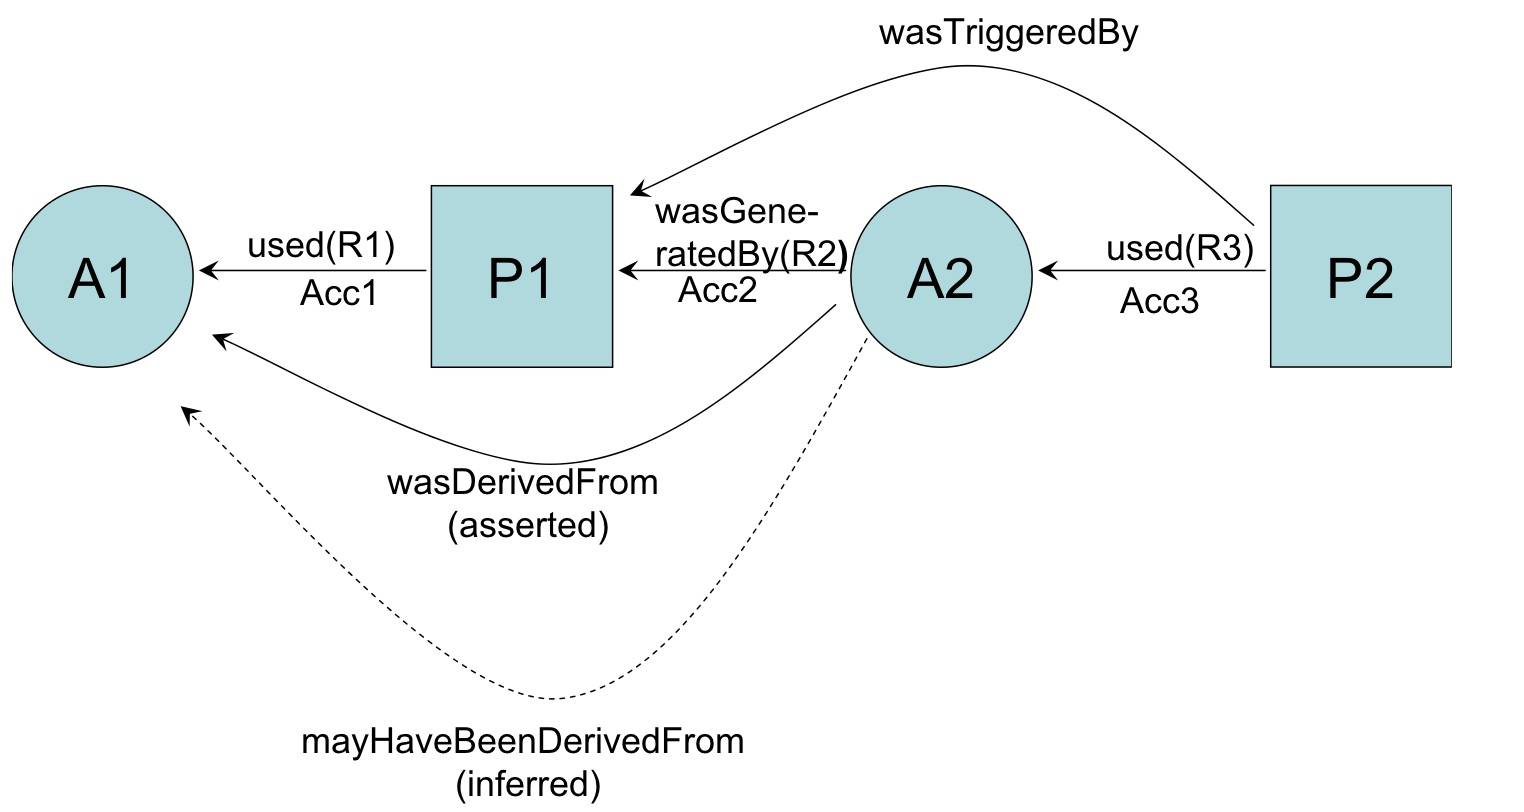
\includegraphics[width=\linewidth]{opm-example.jpg}
    \caption{Ejemplo de un proceso descrito utilizando \textit{OPM}.} Fuente:
    \textit{The Open Provenance Model}.
    \label{fig:opm-example}
\end{figure}

Una vez que hemos definido la procedencia de nuestros datos, podemos definir
otra información relacionada a su fuente tales cómo, autor, certeza de la
información y fuentes para así, a través de un proceso matemático
\cite{dividino2009provenance}, lograr calcular un valor a la confianza de los
datos disponibles. Este proceso, puede ser realizado a múltiples fuentes,
sentencias y grafos, permitiéndonos obtener un valor de confianza para
estructuras más complejas.

\subsubsection{Aplicaciones}
\label{sec:aplicaciones}

El paradigma básico para interactuar con datos es consultar y obtener una
respuesta: los usuarios construyen consultas y los sistemas entregan respuestas.
Por lo tanto, para que un sistema permita a los usuarios interactuar con sus
datos, necesita una interfaz que acepte consultas como entrada y muestre las
respuestas obtenidas desde el sistema de forma visual. En base a esto, muchas de
las actuales interfaces disponibles para interactuar con repositorios
\textit{RDF} o \textit{endpoints SPARQL} corresponden a interfaces interactivas
\textit{web}, como el \href{https://query.wikidata.org}{\textit{Wikidata Query
Service}} donde es posible realizar consultas y visualizar resultados de forma
interactiva (figuras \ref{fig:wikidata-ex-nobel} y
\ref{fig:wikidata-ex-nobel-result}).

\begin{figure}
    \centering
    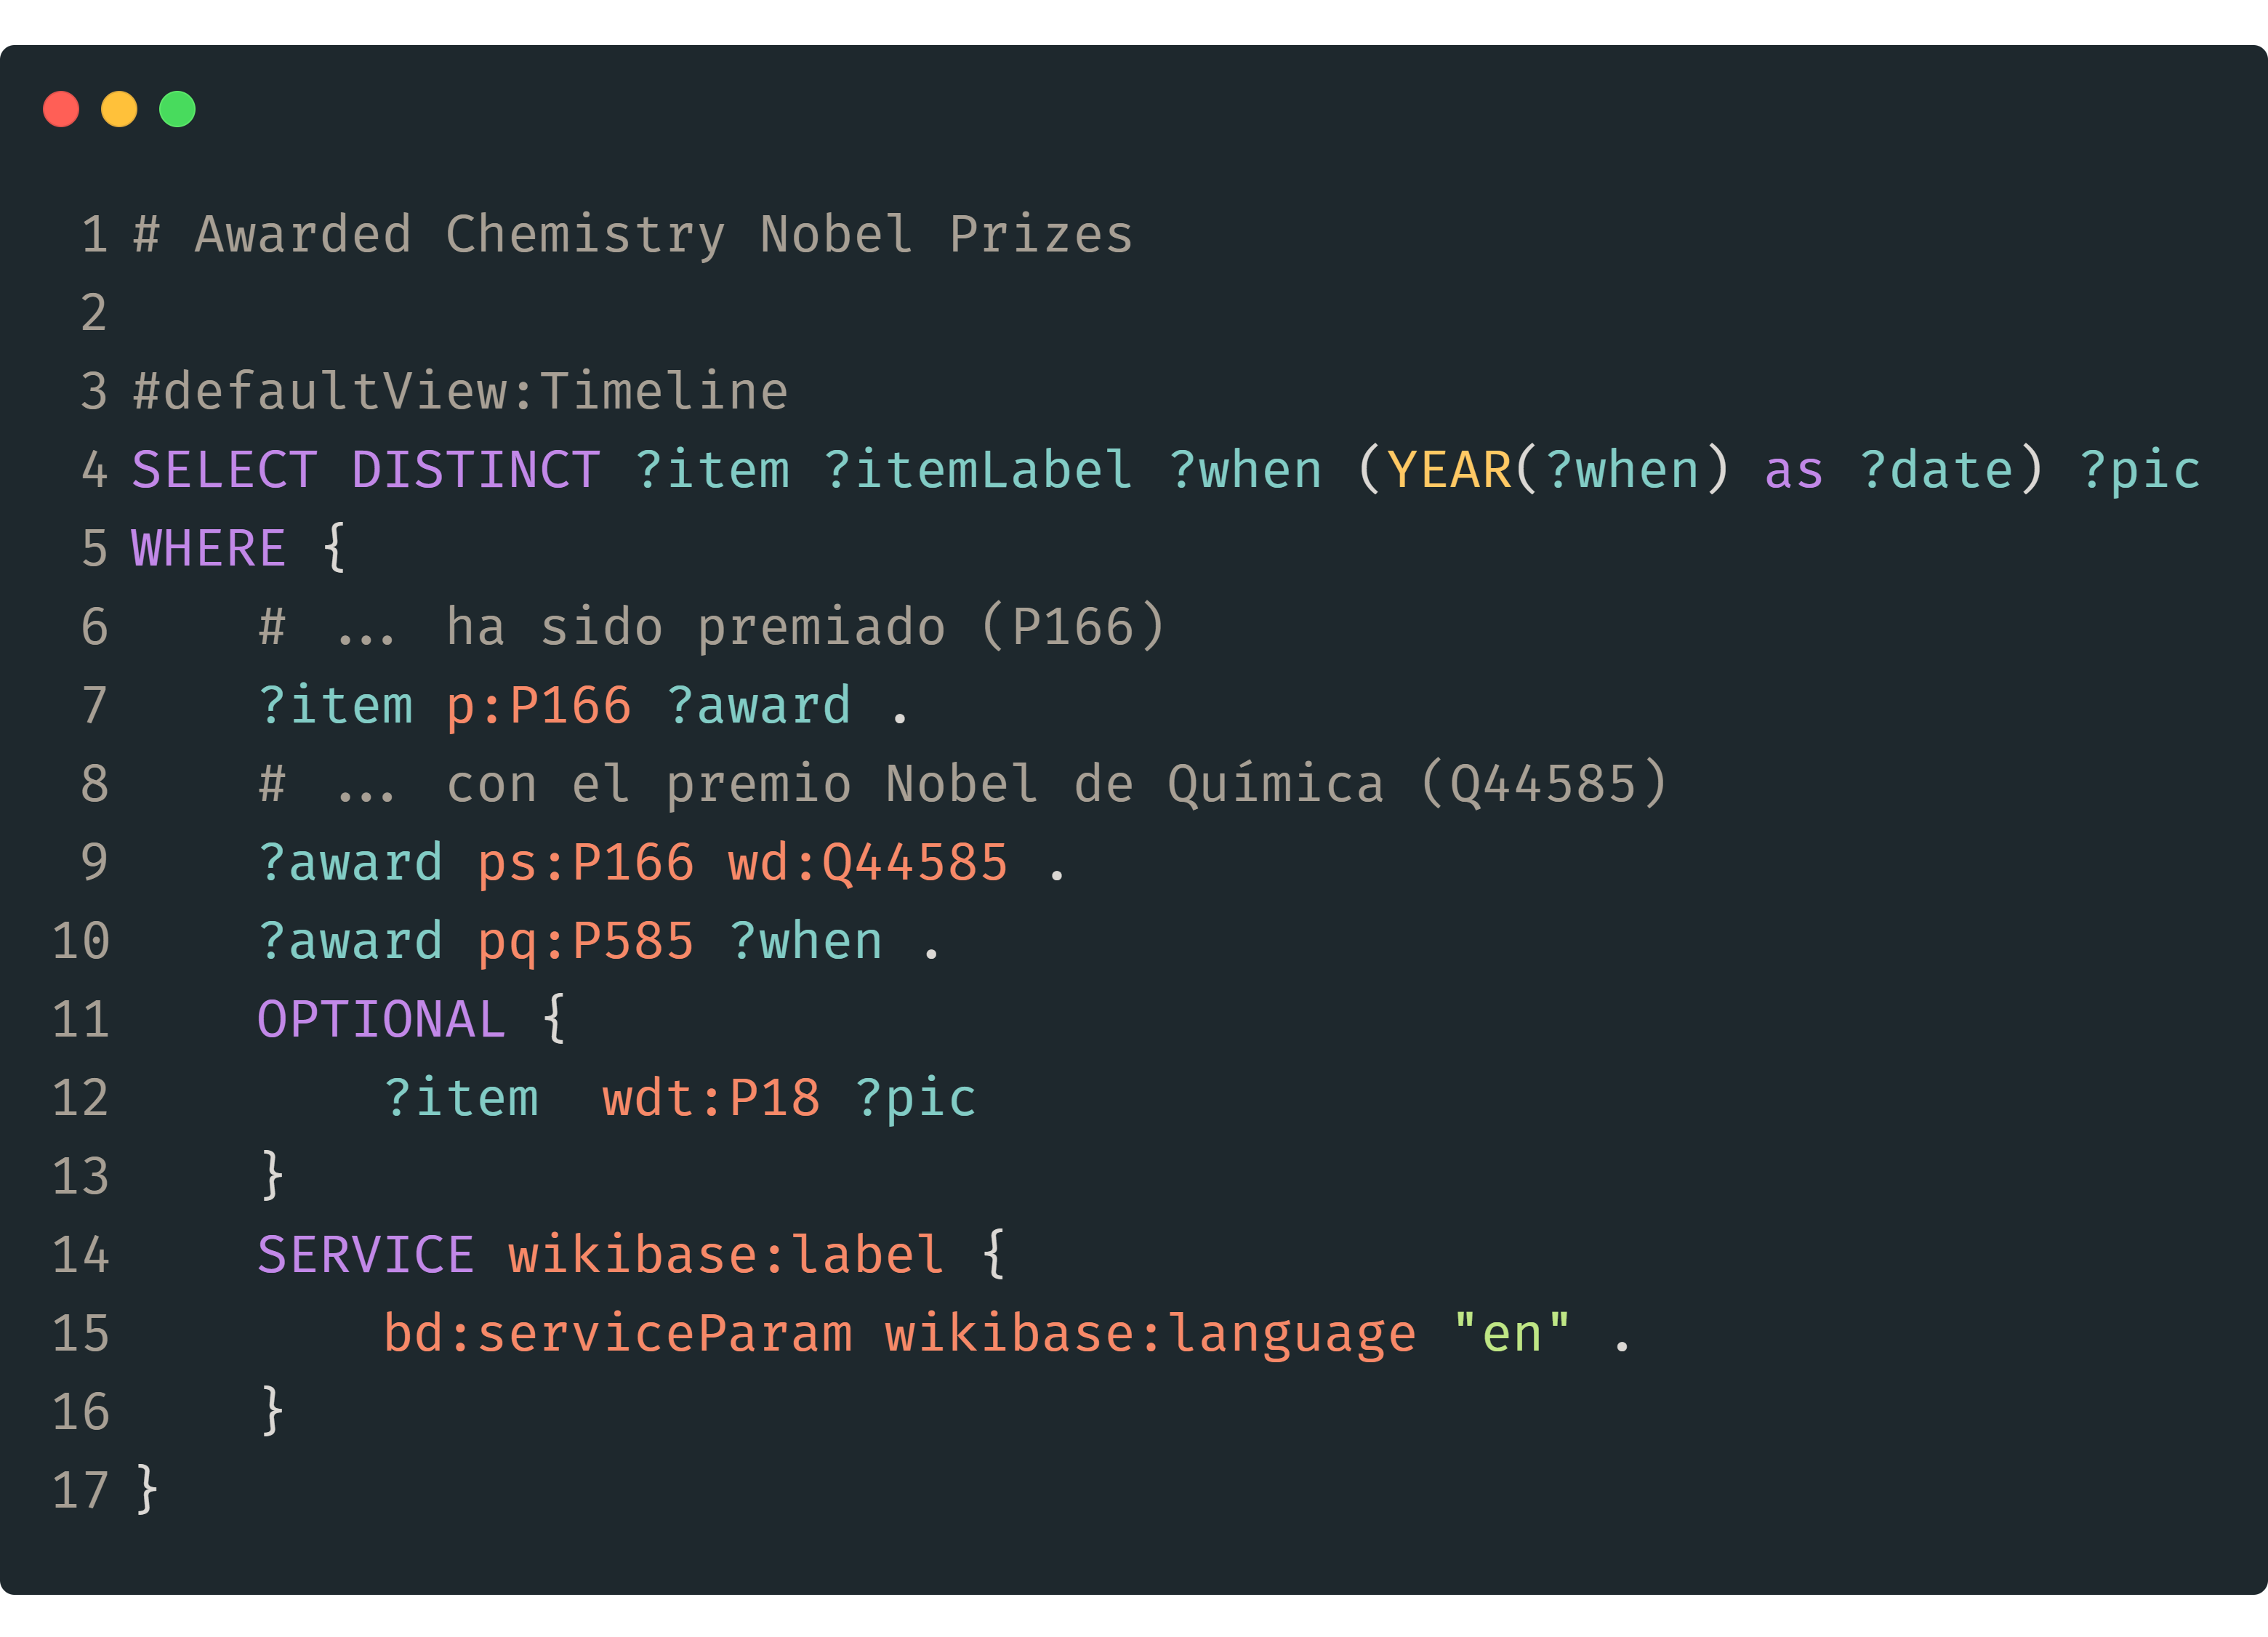
\includegraphics[width=\linewidth]{wikidata-ex-nobel.png}
    \caption{Consulta \textit{SPARQL} realizada en el \textit{Wikidata Query
    Service}.} Corresponde a obtener a aquellas personas que han sido premiadas
    con el Premio Nobel de Química. Fuente: Elaboración propia.
    \label{fig:wikidata-ex-nobel}
\end{figure}

\begin{figure}
    \centering
    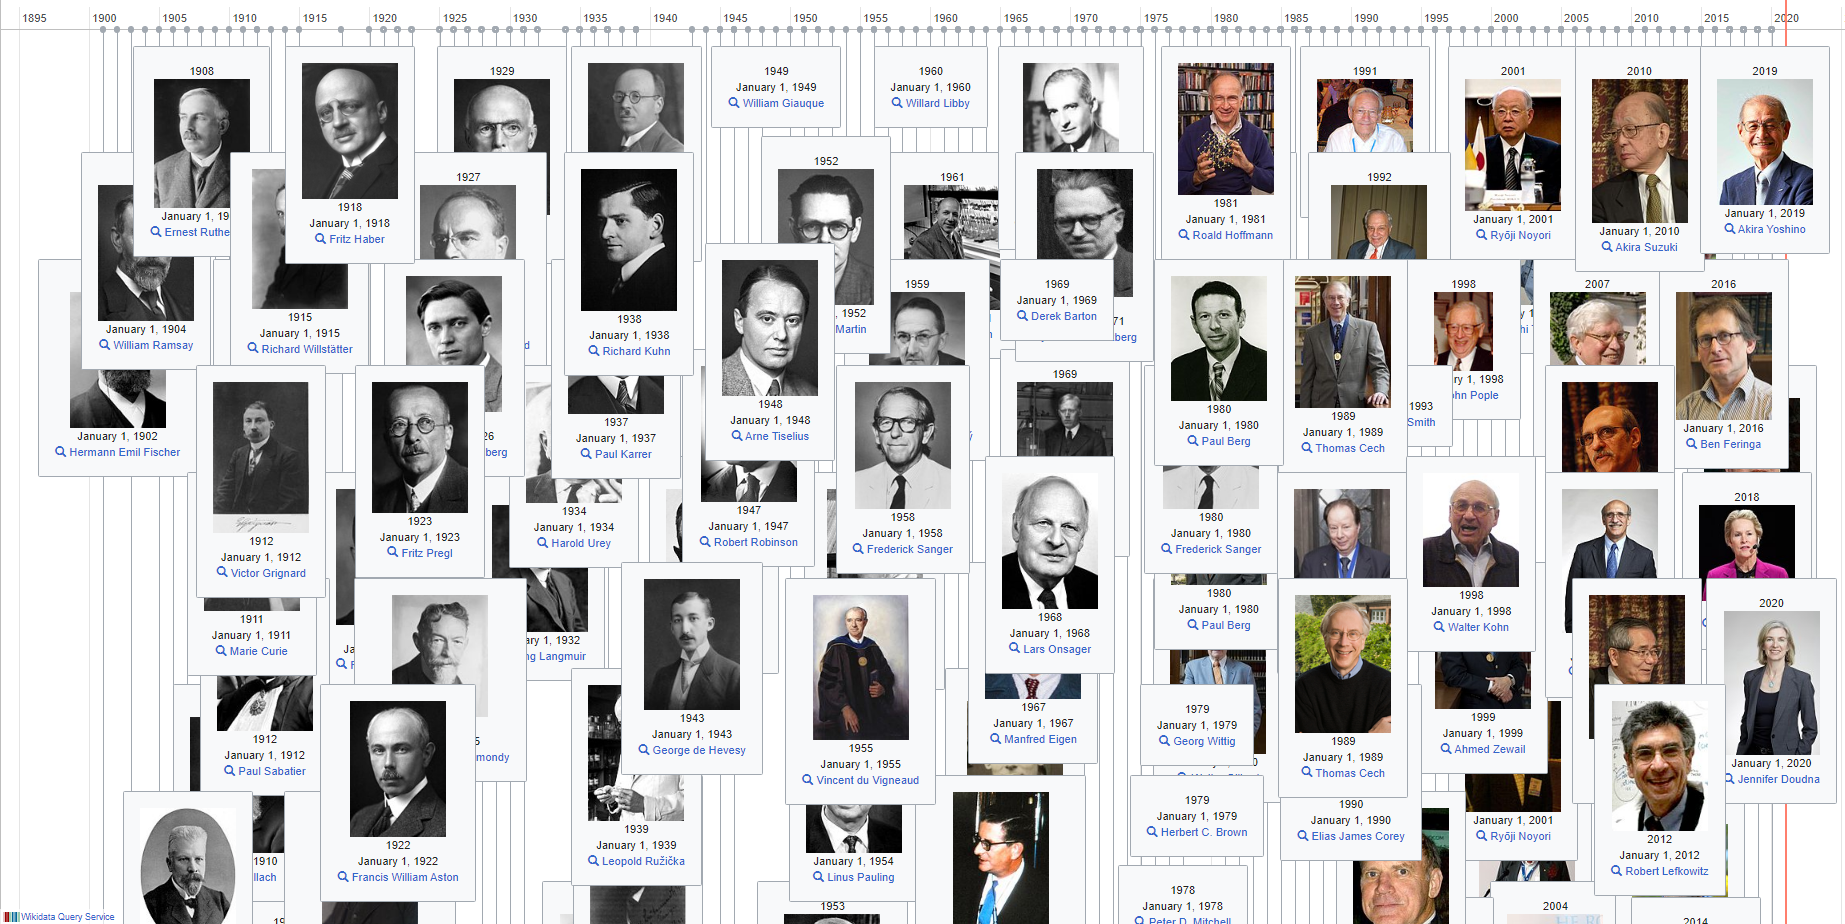
\includegraphics[width=\linewidth]{wikidata-ex-nobel-result.png}
    \caption{Visualización de una consulta \textit{SPARQL} en el
    \textit{Wikidata Query Service}.} Representa los resultados de obtener a
    aquellas personas que han sido premiadas con el Premio Nobel de Química.
    Fuente: \textit{Wikidata Query Service}.
    \label{fig:wikidata-ex-nobel-result}
\end{figure}

La \textit{web} semántica genera nuevos desafíos para el diseño y desarrollo de
interfaces que sean fácil de utilizar para usuarios sin conocimientos técnicos y
que permitan responder a preguntas del estilo ``¿Qué tipo de música se escucha
en las estaciones de radio de Alemania?'' o ``¿Qué personas han participado en
la realización de películas sobre viajes en el tiempo?'' de forma rápida y
fluida.

En base a todas estas definiciones realizadas desde la sección
\ref{sec:refs-transporte-enlazados} hasta la sección \ref{sec:aplicaciones} es
que ahora podemos comprender que es la web semántica y resumirla como el
conjunto de herramientas, lenguajes, protocolos y estándares que permiten tanto
a humanos como a agentes inteligentes procesar toda la información disponible en
la \textit{web} a través de una base de datos global y distribuida.

\subsection{Generación de sugerencias}

El proceso de generación de sugerencias de entidades en base a consultas
\textit{SPARQL} parciales es la interfaz principal a nuestro sistema. Sin
embargo, para realizar este proceso, debemos ser capaces de conocer las
relaciones disponibles en nuestro conjunto de datos sin consultar directamente
al repositorio fuente. Para esto, crearemos un repositorio local que contendrá
las entidades, identificadores, descripciones, relaciones y otras propiedades
necesarias para enviar las sugerencias a nuestros usuarios utilizando el
proyecto \textit{Apache Lucene} \cite{apache2012welcome}. Además, debido a la
gran cantidad de relaciones que pueden existir entre las entidades disponibles,
debemos generar un mecanismo que nos permita ordenar nuestros resultados por
relevancia. Utilizaremos el algoritmo \textit{PageRank} \cite{page1999pagerank}
para realizar este proceso.

\subsubsection{Indexación de documentos}
\label{sec:index-types}

Al buscar información sobre un documento de texto utilizando palabras claves,
estamos realizando una búsqueda sobre el contenido de este texto. Para lograr
esto, necesitamos almacenar información sobre el contenido que estamos revisando
junto con la relación que indica como resultado, el identificador único de la
fuente. Por ejemplo, cuando buscamos un libro a través del nombre de uno de sus
capítulos, las palabras claves son aquellas que se encuentran en el nombre del
capítulo y el identificador puede ser el nombre del libro. Este proceso de
búsqueda se suele realizar a través de índices en bases de datos relacionales.

En el contexto de las bases de datos relacionales, los tipos de indicies más
conocidos son el índice delantero (\textit{forward index}) y en índice inverso
(\textit{inverse index}). Estrictamente hablando, no existe una diferencia
técnica en estos dos tipos de índices, puesto que la implementación es la misma
y es al momento de contextualizar el entorno en el que utilizaremos estos
índices donde se genera una diferencia. En el mundo de la búsqueda de
documentos, un \textit{forward index} se construye describiendo la relación
``El documento \texttt{id=doc1} contiene las palabras \texttt{el} y
\texttt{contenido}'', en cambio, un \textit{inverse index} nos presenta la
información de la forma ``La palabra \texttt{contenido} se encuentra en los
documentos \texttt{id=[doc1, doc2]}''. Una ilustración de este ejemplo se puede
observar en la figura \ref{fig:forward-backward-index}.

\begin{figure}
    \centering
    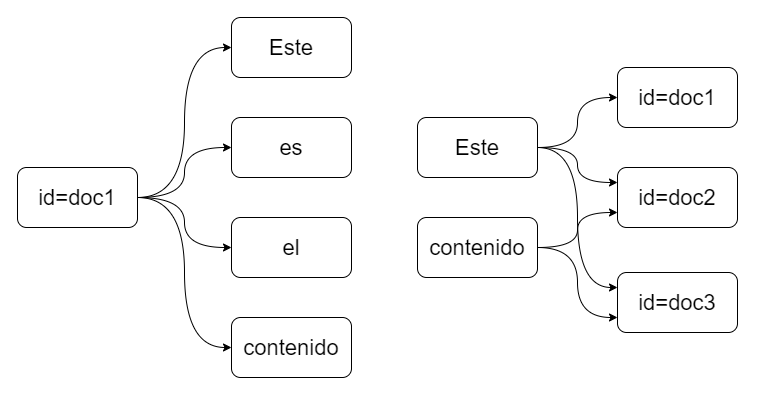
\includegraphics[width=\linewidth]{forward_backward_index.png}
    \caption{Ejemplos de un \textit{forward index} y un \textit{inverted
    index}.} A la izquierda \textit{forward index} y a la derecha
    \textit{inverted index}. Fuente: Elaboración propia.
    \label{fig:forward-backward-index}
\end{figure}

Nuestro repositorio local consiste en un \textit{inverse index}, en el cual, las
etiquetas, descripciones, propiedades y relaciones descritas en el grafo
\textit{RDF} apuntan al identificador de la entidad descrita. De esta forma,
podemos buscar entidades utilizando sus propiedades de la misma forma en la que
buscamos un libro a través de su contenido.

Utilizaremos el proyecto \textit{Apache Lucene} \cite{apache2012welcome} para
lograr esta funcionalidad, puesto que, soporta estos y muchos tipos más de
índices para documentos de texto.

\subsubsection{\textit{Ranking} de resultados}

Una vez que hemos obtenido entidades para generar sugerencias, debemos entregar
a nuestro usuario las más relevantes para la consulta parcial que estamos
construyendo. Para esto, utilizaremos el algoritmo \textit{PageRank}
\cite{page1999pagerank}, el cual nos permite asignar un valor de importancia a
los resultados en base a la cantidad de conexiones que cada elemento del grafo
\textit{RDF} tiene con relación a sus propiedades y otras entidades.

\textit{PageRank} fue diseñado para agregar orden e importancia a los resultados
de los primeros motores de búsqueda en la \textit{web}. En el diseño del
algoritmo, los autores proponen que los sitios disponibles en la \textit{web}
están pueden ser modelados utilizando un grafo dirigido, en el cual, cada sitio
es un nodo del grafo y cada enlace hacia o desde estos sitios representa un arco
entre los nodos. Una vez que hemos construido nuestra representación, debemos
ejecutar nuestro algoritmo recursivo para asignar una alta importancia a
aquellos documentos que tienen muchos enlaces entrantes y pocos enlaces
salientes.

El proceso recursivo asigna un valor inicial al \textit{rank} todos los
documentos en la representación de forma tal que la suma de todos estos valores
es $1$. El siguiente paso es compartir el \textit{rank} de un documento entre
aquellos documentos a los que enlaza: un documento con alto \textit{rank}
entregará bastante puntaje a sus enlazados en comparación a un documento de bajo
\textit{rank} y con muchos enlaces salientes. Este proceso recursivo está
asegurado para converger, por lo que después de una cantidad de terminada de
iteraciones, el \textit{rank} de todos los documentos ha sido calculado.

El valor calculado por \textit{PageRank} es asignado los documentos almacenados
por \textit{Lucene} a través de un \textit{Document level
boosting}\footnote{\textit{Boosting:} Del inglés impulsar. En nuestro contexto,
se refiere a aumentar la importancia de una determinada variable a través de un
mecanismo externo.} el cual es aplicado a cada documento antes de ser ingresado
a nuestro \textit{reverse index} mencionado anteriormente.

% \subsection{\textit{RDFExplorer}}
% 
% \textit{RDFExplorer} es...
% 
% \subsection{\textit{SPARQLforHumans}}
% 
% \textit{SPARQLforHumans} es...

\newpage
\secnumbersection{PROPUESTA DE SOLUCIÓN}

% En esta sección (??)

\subsection{Metodología de trabajo}
\label{sec:metod-de-trabajo}

Para nuestro proyecto, buscaremos utilizar una metodología de trabajo orientada a la agilidad. Existen multiples metodologias de este estilo, pero hemos decidido utilizar el ciclo \textit{PDCA}\footnote{PDCA: Del inglés Planear, Hacer, Verificar, Actuar.} (\textit{Plan}, \textit{Do}, \textit{Check}, \textit{Act}) por las siguientes razones.

\begin{itemize}
    \item \textbf{Simple}. Nuestro mayor motivo es que consiste en un proceso simple, directo e intuitivo que podemos adoptar e implementar en nuestro flujo de trabajo, desarrollo e implementación de la solución.
    \item \textbf{Cilcico}. Debido a la naturaleza ciclica e iterativa, \textit{PDCA} nos permite identificar las causas de los posibles errores durante el proceso de desarrollo del proyecto. Además, a medida que se implementan distintas soluciones es posible obtener información y experiencia para comprender el proceso que se busca mejorar.
    \item \textbf{Adaptable}. Esta metodología es una estrategia muy adaptable, aquellas personas que decidan implementarla puede decidir con total libertad que aspectos se deben considerar en cada una de las etapas del ciclo, la unica condición es que las definiciones se deben mantener a lo largo de todo el proceso. Esta adaptabilidad permite que \textit{PDCA} sea altamente esacalable, ya que se puede adaptar a cualquier situación y en organizaciones de cualquier tamaño, incluso, en equipos de una sola persona.
\end{itemize}

\begin{figure}[ht]
    \centering
    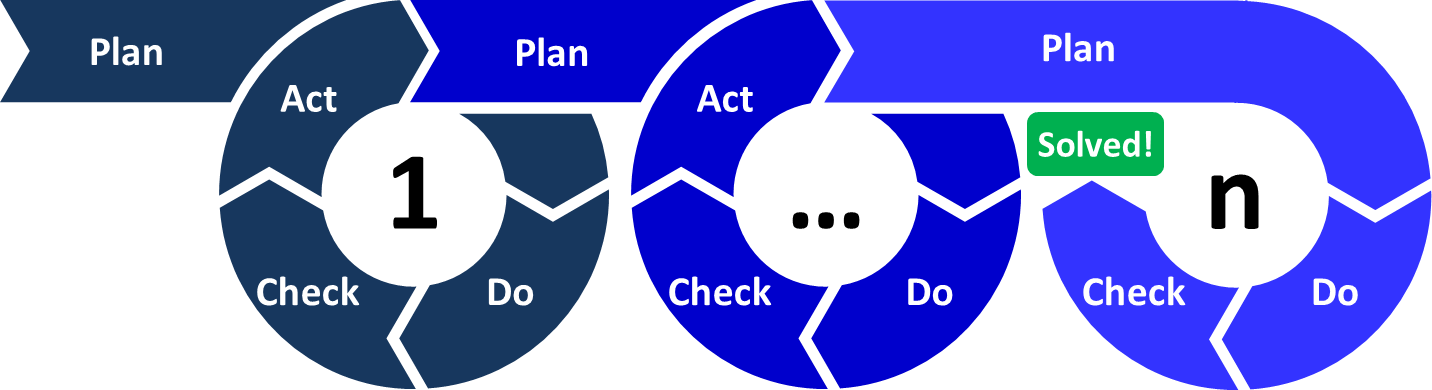
\includegraphics[width=\linewidth]{PDCA-Multi-Loop.png}
    \caption{Ciclos \textit{PDCA}.} Multiples iteraciones del ciclo \textit{PDCA} son realizadas hasta que se logra resolver el problema. Fuente: \textit{PDCA - Wikipedia Commons}.
    \label{fig:pdca-cycle}
\end{figure}

En su esencia \textit{PDCA} es una filosofía para abordar problemas. Primero, identificamos el problema y establecemos nuestros objetivos. Luego, probamos distintos enfoques para alcanzar dichos objetivos, analiszamos nuestros resultados y adaptamos nuestro comportamiento en base a estos. Finalmente, avanzamos la iteración utilizando la solución que ha funcionado.
% TODO: FIXME: REF to https://www.dropbox.com/es/business/resources/pdca

Cada ciclo \textit{PDCA} consiste en las siguientes etapas.

\begin{itemize}
    \item \textbf{Planear}. Debemos comprender nuestro estado actual y el estado deseado. En pocas palabras, esta estapa busca que definamos nuestros objetivos, el cómo alcanzarlos y cómo medir nuestro progreso hacia dichos objetivos.
    \item \textbf{Hacer}. Una vez que hemos definido un plan de acción o una potencial solución para un problema, debemos probarla. Este paso es donde debemos poner a prueba los cambios propuestos en la etapa Planear. Sin embargo, esto se debe considerar como un experimento, no como una solución final. Por lo tanto, todas las pruebas se deben realizar en entornos controlados y a pequeña escala.
    \item \textbf{Verificar}. Luego de completar nuestras pruebas, debemos comprobar que los cambios o soluciones propuestas tienen el efecto deseado. En esta etapa se debe analizar la información recopilada durante la etapa Hacer y comparar lo obtenido con los objetivos y metas originales. En resumen, debemos evaluar nuestro nivel de éxito y qué cosas vamos a conservar para el siguiente paso del ciclo.
    \item \textbf{Actuar}. Al llegar a esta etapa, ya hemos logrado identificar una solución o propuesta de cambio para implementar en nuestro problema o proceso. Se deben aplicar estos cambios en la escala que sea necesaria por el proceso y con esto se definen las bases para una nueva iteración.
\end{itemize}

\subsection{Plan de trabajo}
\label{sec:plan-de-trabajo}

Como hemos mencionado anteriormente, vamos a utilizar cilcos \textit{PDCA} para encontrar la solución a nuestro problema, estos ciclos, son definidos conforme avanzamos en las iteraciones y debido a que se encuentra en el marco de las metodologias agiles, seria irresponsable definir con antelación los objetivos de cada ciclo. Sin embargo, podemos definir determinados hitos que buscamos lograr durante todo este proceso, los cuales, detallamos a continuación.

\begin{enumerate}
    \item Entender la arquitectura inicial de la solución existente (\textit{SPARQLforHumans}).
    \item Diseñar y definir una arquitectura acorde a nuestras restricciones.
    \item Reducir significativamente el tiempo necesario para ejecutar la solución.
    \item Diseñar y definir una arquitectura que permita la actualización en tiempo real de los datos utilizados por nuestra solución.
    \item Actualizar los datos de nuestra solución en tiempo real.
    \item Validar la solución a través de pruebas unitarias automatizadas.
\end{enumerate}

Estos hitos, nos permitiran guiar las iteraciones de nuestro proceso \textit{PDCA} y así no perder el rumbo durante la implementación.

Con las definiciones realizadas en las secciones \ref{sec:metod-de-trabajo} y \ref{sec:plan-de-trabajo} tenemos los necesario para comenzar nuestras iteraciones.

\subsection{Primera iteración: Analisis inicial de la solución existente}

\subsubsection*{Planificación}

Para nuestra primera iteración, nuestro objetivo es entender el proceso y los componentes de la aplicación \textit{SPARQLforHumans}, para esto, revisaremos el código fuente disponible de forma publica \cite{parra2020autocompletion}.

\subsubsection*{Implementación}

Comenzaremos con entender el proceso. Al revisar el código fuente de la aplicación, logramos identificar las siguientes etapas.

\begin{enumerate}
    \item Inicio de la aplicación.
    \begin{enumerate}
        \item Lectura de un fichero en el formato de compresión \textit{gzip} \cite{rfc1952} desde \textit{Wikidata}.
        \item Filtro y validación de lineas en formato \textit{N-Triples}.
        \item Creación de objetos \textit{Triple} en base a lineas validas.
        \item Generación de propiedades inversas para determinadas entidades.
        \item Concatenación de lineas validas y nuevas propiedades a nuevo fichero \textit{gzip}.
        \item Ordenar lineas de nuevo fichero en función de la entidad \textit{RDF} observada en cada linea.
    \end{enumerate}
    \item Indexación de entidades.
    \begin{enumerate}
        \item Lectura de nuevo fichero \textit{gzip} generado anteriormente.
        \item Creación de objetos \textit{Triple}.
        \item Generación de documentos en indice \textit{Lucene} en base a propiedades de cada entidad.
    \end{enumerate}
    \item Obtención del valor \textit{PageRank} para entidades.
    \item Indexación de propiedades.
    \begin{enumerate}
        \item Lectura de documentos disponibles en indice \textit{Lucene} para entidades.
        \item Calculo de frecuencias para las propiedades existentes en los distintos documentos.
        \item Generación de documentos en nuevo indice \textit{Lucene} en función de la frecuencia de cada propiedad identificada.
    \end{enumerate}
    \item Sistema en vivo.
    \begin{enumerate}
        \item Ejecución de prueba estadistica y de rendimiento.
        \item Inicio de servidor Web.
    \end{enumerate}
\end{enumerate}

Las interacciones entre cada etapa se puede observar en el diagrama de procesos presentado en la figura \ref{fig:sfh-bpmn} y los componentes identificados se pueden observar en la figura \ref{fig:sfh-componentes}. Además, presentamos la arquitectura actual del sistema en la figura TODO.

\begin{figure}[ht]
    \centering
    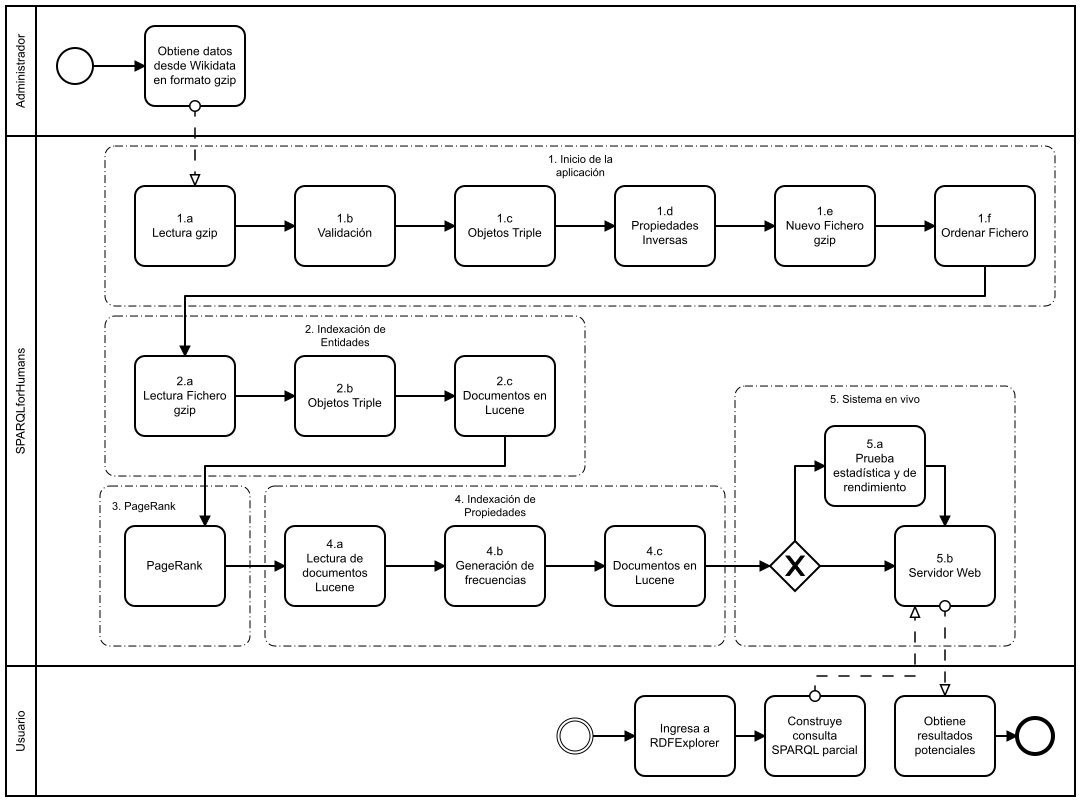
\includegraphics[width=\linewidth]{sparqforhumans_process_bpmn}
    \caption{Proceso de arranque de la aplicación \textit{SPARQLforHumans}.}Fuente: Elaboración Propia.
    \label{fig:sfh-bpmn}
\end{figure}

\begin{figure}
    \centering
    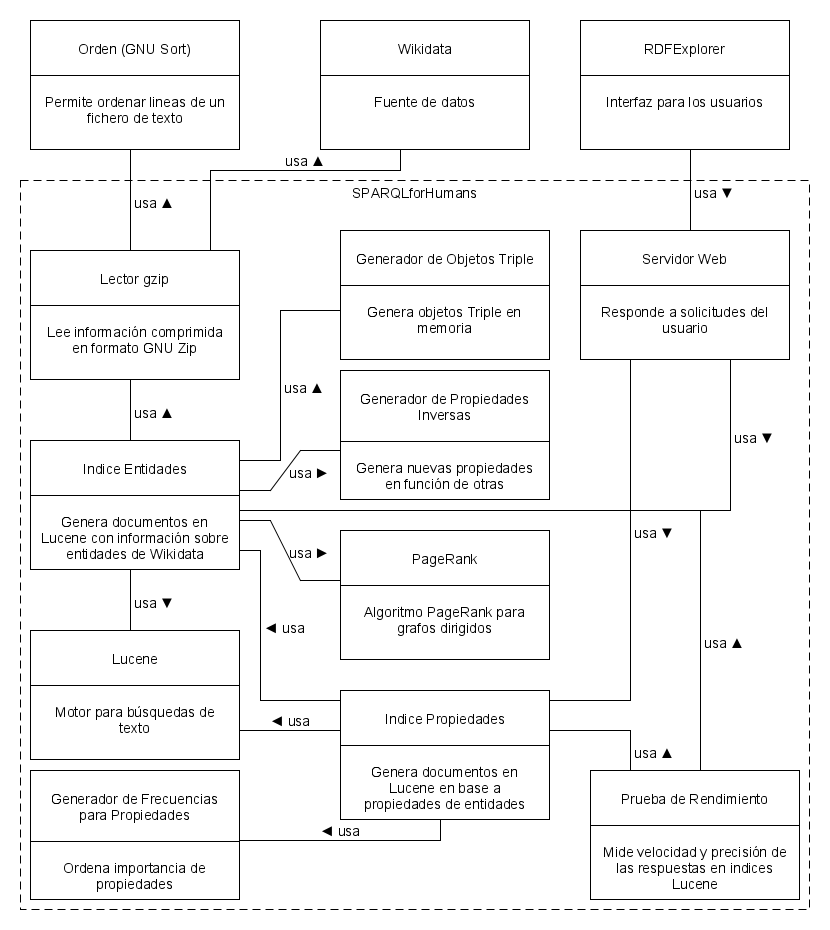
\includegraphics[width=\linewidth]{sfh_comm}
    \caption{Diagrama de componentes para la aplicación \textit{SPARQLforHumans}.}Fuente: Elaboración Propia.
    \label{fig:sfh-componentes}
\end{figure}

\subsubsection*{Resultados}

Gracias al levantamiento de proceso y componentes realizado, podemos ver de forma más clara cómo interactuan cada uno de los distintos modulos de la aplicación existente. Esto nos permite entender su funcionamiento interno, de forma tal, que podemos comenzar a optimizar cada uno de los componentes identificados por separado, acercandonos a nuestro objetivo final.

\subsection{Segunda iteración: Mejoras al rendimiento general}

\subsubsection*{Planificación}

Nuestra segunda iteración consiste en diseñar e implementar el conjunto de mejoras iniciales al rendimiento de la solución. Para lograr esto, comenzaremos con un nuevo diseño y una nueva implementación desde cero, en el lenguaje de programación basado en la \textit{JVM},\footnote{Del inglés. \textit{Java Virtual Machine}.} \textit{Kotlin}\footnote{\textit{The Kotlin Programming Language.} \href{https://kotlinlang.org/}{https://kotlinlang.org/}}. Nuestra implementación se encuentra disponible en un repositorio publico dentro de la plataforma GitHub\footnote{\href{https://github.com/capgadsx/SPARQLforHumans}{https://github.com/capgadsx/SPARQLforHumans}}.

Para esta iteración, definiremos nuestro progreso en función de la cantidad de tiempo reducido en el proceso de arranque de nuestra aplicación. Es decir, desde el punto \texttt{(1.a)} hasta el punto \texttt{(5.b)} de nuestro proceso. Cómo objetivo, hemos definido reducir en al menos un $50\%$ este tiempo de $109$ horas.

\subsubsection*{Implementación}

Comenzaremos aclarando nuestra decisión de utilizar \textit{Kotlin} y la \textit{JVM} para la implementación de nuestra solución. Algo importante a notar es que \textit{SPARQLforHumans} fue escrito utilizando el \textit{.NET Framework} del lenguaje \textit{C\#}, sin embargo, el proyecto \textit{Apache Lucene}\footnote{\href{https://lucene.apache.org/}{https://lucene.apache.org/}} utilizado como el corazón de la solución esta desarrollado en el lenguaje \textit{Java}, por lo que se utiliza una biblioteca de compatibilidad llamada \textit{Lucene.NET}\footnote{\href{https://lucenenet.apache.org/}{https://lucenenet.apache.org/}}. Para nuestra solución, buscamos utilizar el proyecto original, \textit{Apache Lucene}, por lo que deberiamos utilizar \textit{Java}.

Pero no utilizaremos \textit{Java}, como hemos mencionado anteriormente, vamos a utilizar \textit{Kotlin}. \textit{Kotlin} es un lenguaje de programación moderno, maduro y versátil, el cual busca facilitar el desarrollo de aplicaciones. Es consiso, seguro y completamente interoperable con \textit{Java} y otros lenguajes que se ejecutan en la \textit{Java Virtual Machine}. Por lo tanto, podemos utilizar sin problemas todas las funcionalidades de \textit{Apache Lucene} a través de un lenguaje más moderno como \textit{Kotlin}.

Lo siguiente es comentar sobre la implementación realizada. Nuestra solución de referencia corresponde a un sistema monolítico y para nuestras primeras mejoras vamos a seguir este modelo de arquitectura. En resumen, hemos realizado lo siguiente.

\begin{itemize}
    \item Hemos eliminado el modulo de orden. En vez de ordenar nuestros resultados al final del subproceso \texttt{(1)}, vamos a utilizar una estructura de datos llamada \textit{TreeMap},\footnote{\textit{TreeMap}: Un diccionario llave-valor, el cual, al ser recorrido de forma lineal entrega sus llaves de forma ordenada. \href{https://docs.oracle.com/javase/8/docs/api/java/util/TreeMap.html}{https://docs.oracle.com/javase/8/docs/api/java/util/TreeMap.html}} la cual nos permite mantener ordenados las propiedades inversas y objetos \textit{Triple} generados en base al identificador de la entidad que actualmente estamos procesando, cómo por ejemplo $Q88618255$, sin la necesidad de utilizar una herramienta externa como \textit{gzip} o \textit{sort}. Este cambio nos permite eliminar las etapas \texttt{(1.e)} y \texttt{(1.f)} de nuestra nueva solución.
    \item Hemos modernizado el componente que interactua con \textit{Lucene}, utilizando la ultima versión disponible para el formato de indices y la clase \textit{MMapDirectory}\footnote{\href{https://lucene.apache.org/core/8\_9\_0/core/org/apache/lucene/store/MMapDirectory.html}{https://lucene.apache.org/core/8\_9\_0/core/org/apache/lucene/store/MMapDirectory.html}} para interactuar con estos, la cual, corresponde a una interfaz de alto rendimiento que logra aprovechar el \textit{cache} del sistema operativo donde se ejecuta.
    \item Hemos utilizado la biblioteca \textit{Apache Jena}\footnote{\href{https://jena.apache.org/}{https://jena.apache.org/}} para generar objetos \textit{Triple}, esto nos permite generar nuevas propiedades y \textit{Triples} de forma sencilla.
    \item El resto de componentes, han sido implementados en \textit{Kotlin} sin cambios significativos con la implementación de referencia.
\end{itemize}

Para realizar nuestras pruebas y obtener resultados, hemos definido los siguientes ambientes.

\begin{enumerate}
    \item Ambiente de desarrollo.
    \begin{itemize}
        \item Conjunto de datos: \textit{200MB} de datos \textit{N-Triple} comprimidos en formato \textit{gzip}.
        \item Recursos.
        \begin{itemize}
            \item \textit{CPU}. Intel(R) Core(TM) i5-7200U CPU @ 2.50GHz, 4 nucleos.
            \item \textit{RAM}. \textit{7GB}.
            \item Almacenamiento. Samsung SSD 960 EVO 250GB. Interfaz NVME.
        \end{itemize}
    \end{itemize}
    \item Ambiente de pruebas.
    \begin{itemize}
        \item Conjunto de datos: \textit{1GB} de datos \textit{N-Triple} comprimidos en formato \textit{gzip}.
        \item Recursos.
        \begin{itemize}
            \item \textit{CPU}. Intel(R) Core(TM) i5-3470 CPU @ 3.20GHz, 4 nucleos.
            \item \textit{RAM}. \textit{10GB}.
            \item Almacenamiento. Seagate 320GB 7.2K SATA 3.5 HDD.
        \end{itemize}
    \end{itemize}
    \item Ambiente de producción.
    \begin{itemize}
        \item Conjunto de datos: \textit{45GB} de datos \textit{N-Triple} comprimidos en formato \textit{gzip}.
        \item Recursos, (Amazon AWS EC2 Instance - t3.2xlarge).
        \begin{itemize}
            \item \textit{CPU}. Intel(R) Xeon(R) Platinum 8259CL CPU @ 2.50GHz, 8 nucleos.
            \item \textit{RAM}. \textit{32GB}.
            \item Almacenamiento. Amazon AWS EBS, General Purpose SSD (gp2) 200GB. Interfaz NVME.
        \end{itemize}
    \end{itemize}
\end{enumerate}

Al realizar pruebas en pequeña escala, los resultados son alentadores, pero hemos notado un problema, no estamos utilizando de forma eficiente los recursos disponibles de nuestro entorno de ejecución, especialmente nuestra memoria \textit{RAM}.

En la figura \ref{fig:i2-prof-htop}, podemos notar que solo estamos utilizando un $25\%$ de nuestra \textit{CPU} disponible y una gran parte de la memoria \textit{RAM} del sistema, durante toda la ejecución de nuestra aplicación.

\begin{figure}[ht]
    \centering
    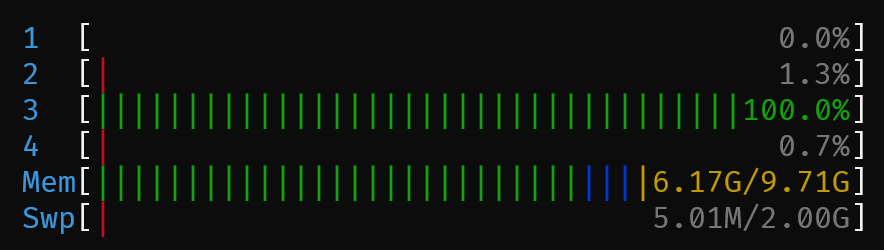
\includegraphics[width=\linewidth]{profiler-memoria-cpu1.png}
    \caption{Utilización de recursos, \textit{CPU} y \textit{RAM} en ambiente de desarrollo.}Fuente: Elaboración Propia.
    \label{fig:i2-prof-htop}
\end{figure}

A pesar de esto, hemos decidido ejecutar el proceso en el ambiente de producción, para así obtener una metrica sobre el tiempo de arranque de nuestra solución. Lamentablemente, solo logramos obtener un error del tipo \textit{java.lang.OutOfMemoryError} despues de unas cuantas horas de ejecución.

La excepción \textit{java.lang.OutOfMemoryError} es un indicador común de una fuga de memoria. Normalmente, este error se genera cuando no hay espacio suficiente para asignar un objeto en el \textit{stack}\footnote{TODO.} de la \textit{JVM}. En este caso, el recolector de basura no puede hacer espacio disponible para acomodar un nuevo objeto, y el \textit{heap}\footnote{TODO.} no puede expandirse más. También, este error puede ser lanzado cuando no hay suficiente memoria nativa para soportar la carga de una nueva clase en la \textit{JVM}. En un casos extremadamente raros, un error del tipo \textit{java.lang.OutOfMemoryError} puede ser lanzado cuando se está gastando una cantidad excesiva de tiempo en la recolección de basura y poca memoria está siendo liberada.

En nuestro caso, creemos que este error se debe a que no es posible acomodar nuevos objetos en nuestra memoria. Además, buscamos saber donde estamos utilizando nuestra \textit{CPU}, con el objetivo de implementar potenciales optimizaciones. Para lograr esto, debemos responder las siguientes preguntas.

\begin{enumerate}
    \item ¿Donde se esta utilizando la \textit{CPU}?
    \item ¿Donde se estan creando los objetos que utilizan nuestra memoria \textit{RAM}?
    \item ¿Que objetos son los que se encuentan en nuestra memoria \textit{RAM}?
\end{enumerate}

Esta clase de dudas pueden ser resueltas utilizando un tipo especifico de herramientas. profilers.

Para responder a nuestra primera incognita, podemos utilizar una herramienta llamada \textit{Java Flight Recorder}\footnote{TODO}, la cual, nos permite medir y grabar lo que se esta ejecutando en la \textit{JVM}. Con esta herramienta podemos generar la figura \ref{fig:i2-prof-jfr}, donde se puede observar una lista de métodos junto con el porcentaje del tiempo que fueron ejecutados en referencia al total del tiempo de ejecución de nuestro programa.

\begin{figure}[ht]
    \centering
    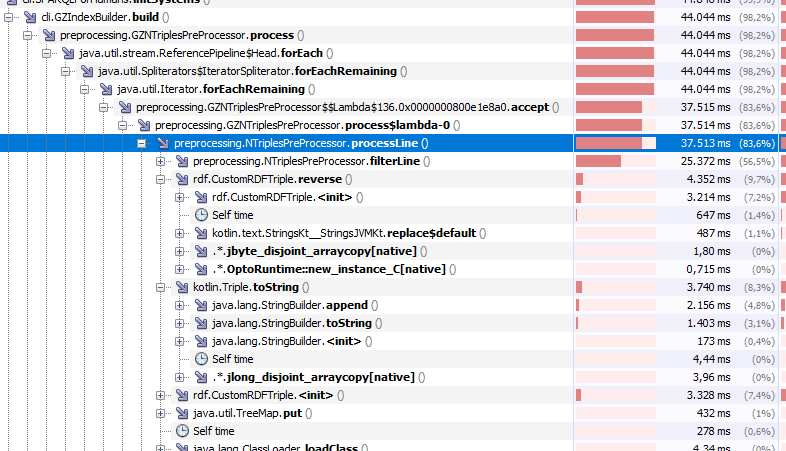
\includegraphics[width=\linewidth]{profiler-string-time.png}
    \caption{Reporte generado por \textit{JFR}.}Fuente: Elaboración Propia.
    \label{fig:i2-prof-jfr}
\end{figure}

Podemos notar, que el $98.2\%$ del tiempo, la \textit{CPU} esta siendo utilizado por el método \texttt{process} de la clase \texttt{GZNTriplesPreProcessor}, el cual, utiliza a \texttt{processLine} y \texttt{filterLine}, ambos de la clase \texttt{NTriplesPreProcessor} y a \texttt{reverse} de la clase \texttt{CustomRDFTriple}. Estos métodos, son los encargados de leer, validar y procesar cada linea del fichero en formato \textit{gzip} utilizado como entrada de nuestra aplicación. Esto significa que no hemos logrado avanzar de las etapas \texttt{(1.b), (1.c)} y \texttt{(1.d)} en nuestra solución.

\begin{figure}[ht]
    \centering
    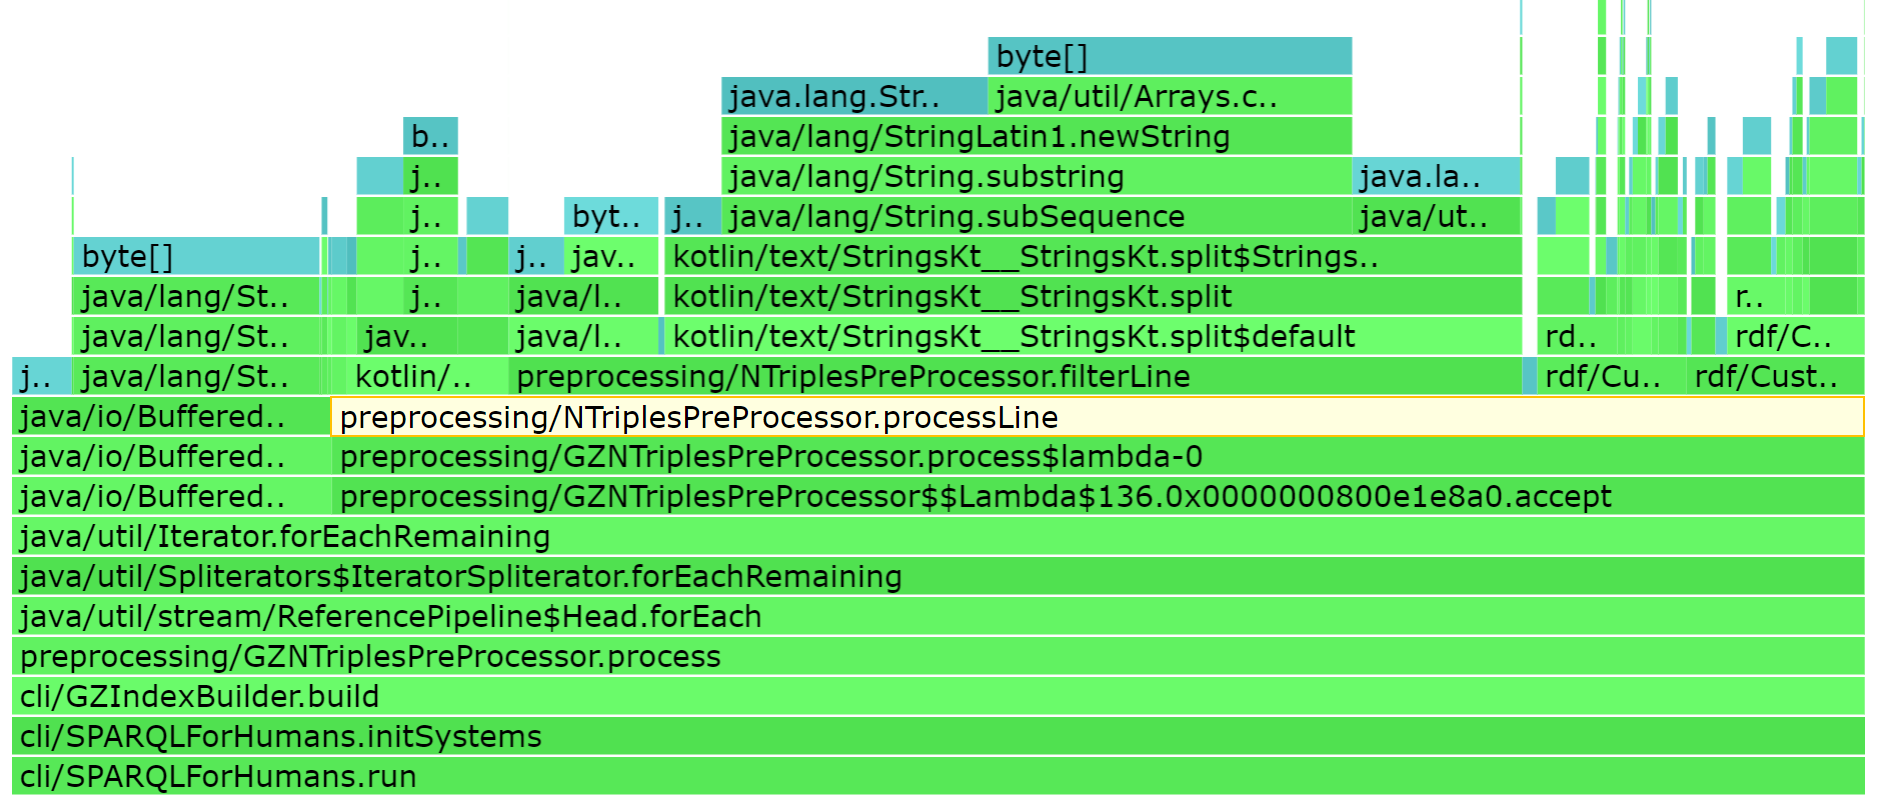
\includegraphics[width=\linewidth]{profiler-mem-flame.png}
    \caption{Reporte generado por \textit{Async-Profiler}.}Fuente: Elaboración Propia.
    \label{fig:i2-prof-mem}
\end{figure}

Para las segunda y tercera preguntas, podemos utilizar el grafico de la figura \ref{fig:i2-prof-mem}, generado por la herramienta \textit{Async-Profiler}\footnote{TODO.}. Esta figura, corresponde a una representación de aquellas funciones que han generado los objetos que se encuentran en la memoria de la \textit{JVM} en un momento determinado. Podemos notar algunos puntos importantes en esta representación.

\begin{itemize}
    \item La mayor parte de los objetos han sido generados desde \texttt{processLine}.
    \item La mayor parte de los objetos corresponden a \texttt{Strings} o \texttt{byte[]}.
    \item Los objetos generados esta fuertemente relacionados a operaciones de separación, subsequencias y concatenación de cadenas de texto (\texttt{String}).
\end{itemize}

Ahora, con el proceso, el código fuente de nuestra implementación y esta nueva información podemos concluir que la causa de nuestro error \textit{java.lang.OutOfMemoryError} es la existencia de multiples objetos del tipo \texttt{String} que no han sido liberados de la memoria durante la ejecución de nuestra solución. Esto se puede observar en más detalle a través de la figura \ref{fig:i2-prof-mem-allocs}.

\begin{figure}[ht]
    \centering
    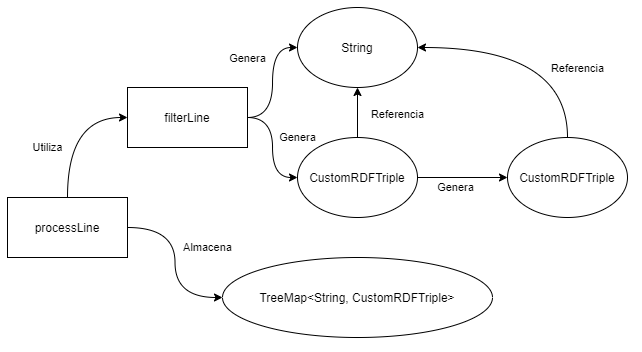
\includegraphics[width=\linewidth]{mem-allocs-jvm.png}
    \caption{Generación de objetos \texttt{CustomRDFTriple}.}Fuente: Elaboración Propia.
    \label{fig:i2-prof-mem-allocs}
\end{figure}

En la figura se puede observar que la función \texttt{processLine} utiliza a \texttt{filterLine} para generar objetos del tipo \texttt{CustomRDFTriple}, el cual a su vez, puede generar otro objeto \texttt{CustomRDFTriple} en función de sus propiedades inversas. Estos, utilizan objetos \texttt{String} para interactuar con la biblioteca \textit{Apache Jena} y obtener determinada información sobre los \textit{Triples} que representan. Aquellos \texttt{Strings} son almacenados como propiedades de los \texttt{CustomRDFTriples}. Finalmente, ambos \texttt{CustomRDFTriples} son almacenados de forma ordenada en una instancia \texttt{TreeMap}.

Toda esta nueva información sobre las necesidades funcionales de la aplicación nos hacen cuestionar la decisión de utilizar \textit{Kotlin} y la \textit{JVM} para procesar grandes cantidades de texto.

\subsubsection*{Resultados}

No hemos logrado nuestro objetivo en esta iteración, debido a que no logramos ejecutar completamente nuestra solución. Sin embargo, no todo es malas noticias, hemos obtenido información valiosa para continuar en el desarrollo de la solución. En resumidas cuentas, lo siguiente.

\begin{itemize}
    \item Debemos realizar una implementación que utilize una menor cantidad de memoria \textit{RAM} del sistema.
    \item Debemos paralelizar nuestra solución, de esta forma, utilizaremos de forma más eficiente nuestra \textit{CPU} y lograremos acercarnos aún más a nuestro objetivo.
    \item Existe una optimización importante en la etapa \texttt{(3 - PageRank)}, puesto que, se está utilizando una implementación iterativa del algoritmo. Funciona en pequeña escala, pero al utilizar una cantidad real de $90$ millones de nodos, definitivamente nos va a tomar tiempo procesar todo.
\end{itemize}

Con toda esta nueva información y nuevas necesidades, estamos listos para volver a intentar alcanzar nuestro objetivo de reducir en un $50\%$ nuestro tiempo de arranque en una nueva iteración.

\subsection{Tercera iteración: Desacoplamiento de componentes, \textit{Message Brokers} y codificación binaria}

\subsubsection*{Planificación}

A

\subsubsection*{Implementación}

A

\subsubsection*{Resultados}

A

\subsection{Cuarta iteración: Paralelización de etapas}

\subsubsection*{Planificación}

A

\subsubsection*{Implementación}

A

\subsubsection*{Resultados}

A

\subsection{Quinta iteración: Actualización de resultados en tiempo real}

\subsubsection*{Planificación}

A

\subsubsection*{Implementación}

A

\subsubsection*{Resultados}

A

\subsection{Sexta iteración: Optimizaciones de transporte}

\subsubsection*{Planificación}

A

\subsubsection*{Implementación}

A

\subsubsection*{Resultados}

A

\subsection{Septima iteración: Implementación de pruebas}

\subsubsection*{Planificación}

A

\subsubsection*{Implementación}

A

\subsubsection*{Resultados}

A


\newpage
\input{validacion_de_la_solucion}
\newpage
\secnumbersection{CONCLUSIONES}

Las Conclusiones son, según algunos especialistas, el aspecto principal de una memoria, ya que reflejan el aprendizaje final del autor del documento. En ellas se tiende a considerar los alcances y limitaciones de la propuesta de solución, establecer de forma simple y directa los resultados, discutir respecto a la validez de los objetivos formulados, identificar las principales contribuciones y aplicaciones del trabajo realizado, así como su impacto o aporte a la organización o a los actores involucrados. Otro aspecto que tiende a incluirse son recomendaciones para quienes se sientan motivados por el tema y deseen profundizarlo, o lineamientos de una futura ampliación del trabajo.

\underline{Todo esto debe sintetizarse en al menos 5 páginas.}

FIXME: CONCLUSIONES P1

\newpage
FIXME: CONCLUSIONES P2

\newpage
FIXME: CONCLUSIONES P3

\newpage
FIXME: CONCLUSIONES P4

\newpage
FIXME: CONCLUSIONES P5

\newpage
\input{anexos}

\newpage
% Bibliografía estilo APA:
\bibliographystyle{apalike-es}
\bibliography{bibliografia}{}

\end{document}
